% Options for packages loaded elsewhere
\PassOptionsToPackage{unicode}{hyperref}
\PassOptionsToPackage{hyphens}{url}
\PassOptionsToPackage{dvipsnames,svgnames,x11names}{xcolor}
%
\documentclass[
  letterpaper,
  DIV=11,
  numbers=noendperiod]{scrartcl}

\usepackage{amsmath,amssymb}
\usepackage{iftex}
\ifPDFTeX
  \usepackage[T1]{fontenc}
  \usepackage[utf8]{inputenc}
  \usepackage{textcomp} % provide euro and other symbols
\else % if luatex or xetex
  \usepackage{unicode-math}
  \defaultfontfeatures{Scale=MatchLowercase}
  \defaultfontfeatures[\rmfamily]{Ligatures=TeX,Scale=1}
\fi
\usepackage{lmodern}
\ifPDFTeX\else  
    % xetex/luatex font selection
\fi
% Use upquote if available, for straight quotes in verbatim environments
\IfFileExists{upquote.sty}{\usepackage{upquote}}{}
\IfFileExists{microtype.sty}{% use microtype if available
  \usepackage[]{microtype}
  \UseMicrotypeSet[protrusion]{basicmath} % disable protrusion for tt fonts
}{}
\makeatletter
\@ifundefined{KOMAClassName}{% if non-KOMA class
  \IfFileExists{parskip.sty}{%
    \usepackage{parskip}
  }{% else
    \setlength{\parindent}{0pt}
    \setlength{\parskip}{6pt plus 2pt minus 1pt}}
}{% if KOMA class
  \KOMAoptions{parskip=half}}
\makeatother
\usepackage{xcolor}
\usepackage[top=13mm, bottom=13mm, left=13mm, right=13mm]{geometry}
\setlength{\emergencystretch}{3em} % prevent overfull lines
\setcounter{secnumdepth}{-\maxdimen} % remove section numbering
% Make \paragraph and \subparagraph free-standing
\ifx\paragraph\undefined\else
  \let\oldparagraph\paragraph
  \renewcommand{\paragraph}[1]{\oldparagraph{#1}\mbox{}}
\fi
\ifx\subparagraph\undefined\else
  \let\oldsubparagraph\subparagraph
  \renewcommand{\subparagraph}[1]{\oldsubparagraph{#1}\mbox{}}
\fi


\providecommand{\tightlist}{%
  \setlength{\itemsep}{0pt}\setlength{\parskip}{0pt}}\usepackage{longtable,booktabs,array}
\usepackage{calc} % for calculating minipage widths
% Correct order of tables after \paragraph or \subparagraph
\usepackage{etoolbox}
\makeatletter
\patchcmd\longtable{\par}{\if@noskipsec\mbox{}\fi\par}{}{}
\makeatother
% Allow footnotes in longtable head/foot
\IfFileExists{footnotehyper.sty}{\usepackage{footnotehyper}}{\usepackage{footnote}}
\makesavenoteenv{longtable}
\usepackage{graphicx}
\makeatletter
\def\maxwidth{\ifdim\Gin@nat@width>\linewidth\linewidth\else\Gin@nat@width\fi}
\def\maxheight{\ifdim\Gin@nat@height>\textheight\textheight\else\Gin@nat@height\fi}
\makeatother
% Scale images if necessary, so that they will not overflow the page
% margins by default, and it is still possible to overwrite the defaults
% using explicit options in \includegraphics[width, height, ...]{}
\setkeys{Gin}{width=\maxwidth,height=\maxheight,keepaspectratio}
% Set default figure placement to htbp
\makeatletter
\def\fps@figure{htbp}
\makeatother

\usepackage{booktabs}
\usepackage{longtable}
\usepackage{array}
\usepackage{multirow}
\usepackage{wrapfig}
\usepackage{float}
\usepackage{colortbl}
\usepackage{pdflscape}
\usepackage{tabu}
\usepackage{threeparttable}
\usepackage{threeparttablex}
\usepackage[normalem]{ulem}
\usepackage{makecell}
\usepackage{xcolor}
\KOMAoption{captions}{tableheading}
\makeatletter
\makeatother
\makeatletter
\makeatother
\makeatletter
\@ifpackageloaded{caption}{}{\usepackage{caption}}
\AtBeginDocument{%
\ifdefined\contentsname
  \renewcommand*\contentsname{Table of contents}
\else
  \newcommand\contentsname{Table of contents}
\fi
\ifdefined\listfigurename
  \renewcommand*\listfigurename{List of Figures}
\else
  \newcommand\listfigurename{List of Figures}
\fi
\ifdefined\listtablename
  \renewcommand*\listtablename{List of Tables}
\else
  \newcommand\listtablename{List of Tables}
\fi
\ifdefined\figurename
  \renewcommand*\figurename{Figure}
\else
  \newcommand\figurename{Figure}
\fi
\ifdefined\tablename
  \renewcommand*\tablename{Table}
\else
  \newcommand\tablename{Table}
\fi
}
\@ifpackageloaded{float}{}{\usepackage{float}}
\floatstyle{ruled}
\@ifundefined{c@chapter}{\newfloat{codelisting}{h}{lop}}{\newfloat{codelisting}{h}{lop}[chapter]}
\floatname{codelisting}{Listing}
\newcommand*\listoflistings{\listof{codelisting}{List of Listings}}
\makeatother
\makeatletter
\@ifpackageloaded{caption}{}{\usepackage{caption}}
\@ifpackageloaded{subcaption}{}{\usepackage{subcaption}}
\makeatother
\makeatletter
\@ifpackageloaded{tcolorbox}{}{\usepackage[skins,breakable]{tcolorbox}}
\makeatother
\makeatletter
\@ifundefined{shadecolor}{\definecolor{shadecolor}{rgb}{.97, .97, .97}}
\makeatother
\makeatletter
\makeatother
\makeatletter
\makeatother
\ifLuaTeX
  \usepackage{selnolig}  % disable illegal ligatures
\fi
\IfFileExists{bookmark.sty}{\usepackage{bookmark}}{\usepackage{hyperref}}
\IfFileExists{xurl.sty}{\usepackage{xurl}}{} % add URL line breaks if available
\urlstyle{same} % disable monospaced font for URLs
\hypersetup{
  pdftitle={Journey to Paris 2024: A Bayesian Approach to Finding the Best Men's and Women's U.S. Gymnastics Teams},
  pdfauthor={Chris Liang, Enzo Moraes Mescall, Mitchelle Mojekwu, Zoe Svec},
  colorlinks=true,
  linkcolor={blue},
  filecolor={Maroon},
  citecolor={Blue},
  urlcolor={Blue},
  pdfcreator={LaTeX via pandoc}}

\title{Journey to Paris 2024: A Bayesian Approach to Finding the Best
Men's and Women's U.S. Gymnastics Teams}
\author{Chris Liang, Enzo Moraes Mescall, Mitchelle Mojekwu, Zoe Svec}
\date{}

\begin{document}
\maketitle
\ifdefined\Shaded\renewenvironment{Shaded}{\begin{tcolorbox}[enhanced, frame hidden, interior hidden, borderline west={3pt}{0pt}{shadecolor}, sharp corners, boxrule=0pt, breakable]}{\end{tcolorbox}}\fi

\hypertarget{introduction}{%
\subsection{Introduction}\label{introduction}}

The Olympic Games are a highly anticipated world-renowned multi-sporting
event that takes place every four years. Particularly the Summer Olympic
Games tend to have a wider variety of 32 sports and more viewers than
that of the Winter Olympics (Olympics, 2021). Athletes from all over the
world can participate granted they meet the criteria established by
their nation's Olympic committees and the international sports
federations. With female qualifying gymnasts from the United States
placing with medals in the team all-around, individual all-around, and
each individual apparatus in the 2020 Tokyo Olympics game, there has
been a surge in media attention on the United States gymnastics teams
(Olympics, 2020).

As the Paris 2024 Summer Olympic Games is approaching, the United States
Olympic Men's and Women's Artistic Gymnastics aims to put together a
team of 5 each that best represents the country on the world's sporting
stage by optimizing medal success amongst the team all-around,
individual all-around, and individual apparatus events. At the Paris
Olympics, during the qualifications round, from the 5 team members, 4
will compete on each apparatus, and the 3 highest scores will count and
be summed. In the finals, the top 8 countries will qualify and compete
in team all-around, where from the 5 team members, 3 will compete on
each apparatus and all 3 scores will count. In the individual all-around
finals, 24 athletes will qualify, with maximum 2 athletes per country.
In the individual apparatus finals, 8 athletes will qualify per
apparatus with a maximum of 2 athletes per country. The low number of
athletes that qualify for the finals suggests there must be thoughtful
crafting of the team of 5. This study aims to use the most recent
Olympic Games and other world competitions' qualifying and final round
results data to best assemble a team that is likely to produce optimal
success in terms of medals within the Olympic qualifiers and final
criteria (UCSAS, 2023).

The UConn Sports Analytics Symposium provisioned two clean data sets of
the accumulation of results of teams worldwide that participated in the
major domestic and international gymnastic qualifying and final
competition events leading up to the 2024 Summer Olympic Games. The
first data set includes includes the results of the 2020 (taking place
in 2021) Tokyo Summer Olympics qualifying and final rounds, and the
second data set includes competitions in the 2022 and 2023 seasons.
Observations for both data sets are at the athlete- and apparatus-level
score for an event in a round at a gymnastics competition--for example,
Simone Biles's final uneven bars score at the 2023 US Gymnastics
Championships. It is worth noting, however, that the data from the Tokyo
Olympics only include results for women's gymnastics, while the data
from 2022-2023 include results for both men's and women's gymnastics.
The data are collected from the results on each corresponding
competition's official website, which are results from the officially
judged scores of each competition. Variables in the data sets include
first and last names of each athlete, gender, country, date of
competition, name of competition, the round of the competition
(e.g.~qualifier or final of an individual apparatus, individual
all-around, or team event), the location of the competition, apparatus
(women compete in ``BB'': balance beam, ``FX'': floor exercise, ``UB'':
uneven bars, and ``VT'': vault; men compete in ``FX'': floor exercise,
HB'': high bar, ``PB'': parallel bars, ``PH'': pommel horse, ``SR'':
still rings, ``VT'': vault; beyond the floor and vault overlap, both men
and women may compete in vaults ``VT1'' and ``VT2'', which are 2
different vaults required in individual apparatus qualifications and
finals), the execution score, difficulty score, penalty, and final score
for that athlete on that apparatus, and the rank of that athlete in that
apparatus and round.

We decided to not proceed in using the data set of results from the
Tokyo Summer Olympics since the data consisted only of female athletes
and one competition (the Olympic Games). Additionally, in the context of
Olympic gymnastics, athletes of age 16 and older are eligible to compete
but gymnastics is a sport in which most athletes retire in their early
to mid-twenties. Specifically in the summer 2020 Tokyo Olympics only
three female athletes aged 27 or older qualified to compete (Camenker,
2021). Furthermore, the average age for female gymnasts in the 2020
Olympics was approximately 22 years of age, meaning we assume that many
of the competitors in the older data set will not be competing in the
2024 Paris Summer Olympics (Meyers, 2021).

We have the following objectives for this study: (UCSAS, 2023)

\begin{enumerate}
\def\labelenumi{\arabic{enumi})}
\item
  Decide on whether to maximize total medal count, gold medal count, or
  a weighted medal count (e.g., 3 for gold, 2 for silver, 1 for bronze).
\item
  Decide on whether to value the medals of an event over others. For
  example, consider a team all-around medal to be more valuable than the
  individual all-around medals and/or consider the individual all-around
  medals to be more valuable than the individual apparatus medals.
\item
  Decide on whether Team USA should maximize its total medal count by
  selecting a team of five gymnasts who are all-around gymnasts, event
  specialists (gymnasts who focus on 1 or more apparatus but not all
  apparatus), or a combination of those. This should consider under what
  circumstances can Team USA maximize its total medal count by selecting
  a gymnast who only competes on 1 apparatus (e.g., Stephen Nederoscik,
  2021 pommel horse World Champion).
\item
  Identify the group of five athletes who will most likely enable the
  Team USA Olympic Men's and Women's Artistic Gymnastics team to
  maximize medals won in the Paris 2024 Summer Olympics using an
  analytical model.
\end{enumerate}

Addressing these objectives will assist the national Olympic Artistic
Gymnastics teams in best approaching the Olympic gymnastics events in
totality by offering recommended strategies to best approach team
selection. In our analysis of the best fit US male and female gymnastics
teams for the Paris Olympics, we will undertake a Bayesian approach to
simulate outcomes of individual athletes' scores in an apparatus.
Bayesian frameworks in sports analytics to simulate athlete's results
are well-documented and have seen a rise in popularity in the past
decade (Santos-Fernandez, et. al., 2019). For instance, Yang and Swartz
use Monte Carlo Markov Chains to simulate the outcomes of baseball games
(Yang et. al., 2022). We will build upon these analyses and choose the
appropriate Bayesian method to simulate outcomes of gymnast results in
each apparatus, after which we will analyze the top performers in each
apparatus, assign medals, and find the best combination of athletes.

\hypertarget{exploratory-data-visualizations}{%
\subsubsection{Exploratory Data
Visualizations}\label{exploratory-data-visualizations}}

We created some exploratory data visualizations to examine the
distributions of athlete scores and examine the performance of US
athletes relative to other countries. We find that from the density
plots of male and female athletes' overall scores (difficulty score +
execution score - penalty = overall score) per apparatus that the scores
are approximately normally distributed for the apparatuses for both
genders. There are some slight deviations from normality, namely women's
vault scores and uneven bars scores are slightly skewed left and men's
still rings scores have a slight dip in the peak. Nonetheless, the
approximate normality of the distribution of athlete's scores by
apparatus informs our bayesian approach, as we may use normal priors for
our data. Furthermore, we plotted the number of athletes per country in
the top 10 of each apparatus internationally, top 10 meaning the
athletes with top 10 highest mean scores for each apparatus. For
example, we see that for women's vault, 6 of the top 10 athletes in the
world are US gymnasts. These plots help inform us of if we should be
thinking about specialists or generalists in the US team combinations.
We see that the top 10 for each apparatus have a high concentration of
US female gymnasts, so we may want specialists in our team makeup,
whereas that case does not transfer to the US male gymnasts, as there
are few US male gymnasts in the top 10 for the floor exercise, high bar,
pommel horse, and still rings apparatuses. In the men's case, we may not
want to send specialists to take up a spot on team of five, and we shall
explore this conjecture in our simulations.

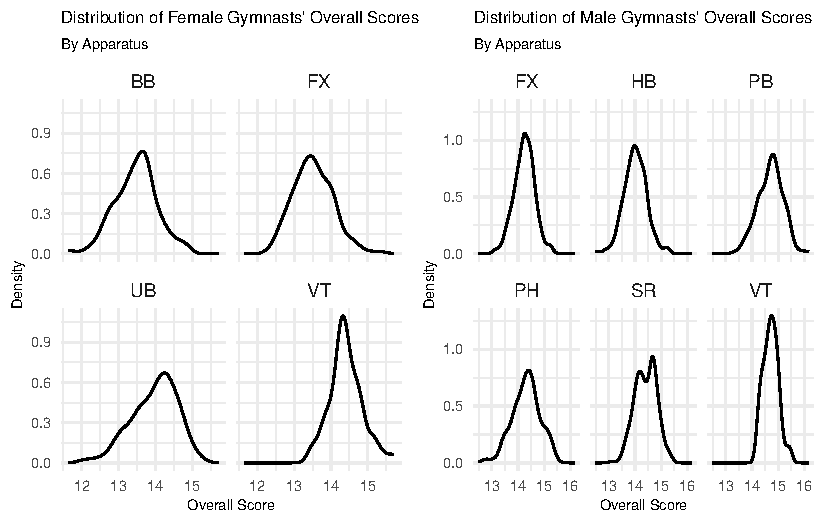
\includegraphics{Main_files/figure-pdf/score-distributions-1.pdf}

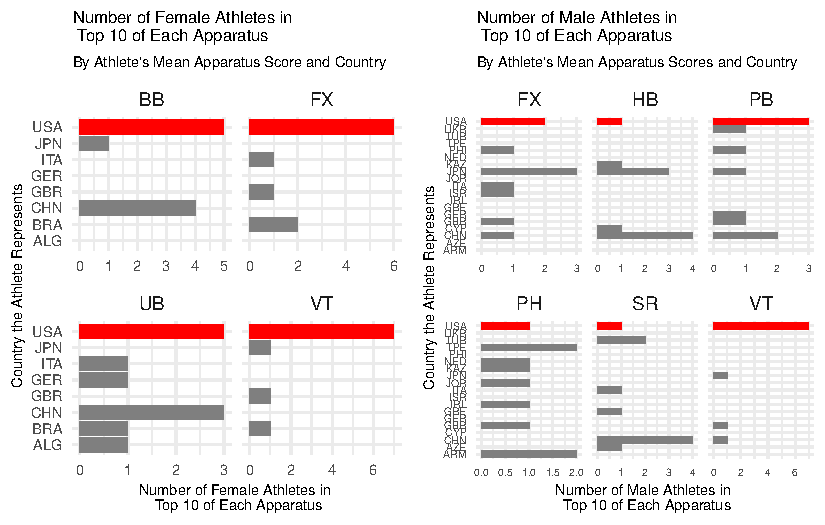
\includegraphics{Main_files/figure-pdf/top-10-athletes-1.pdf}

\hypertarget{methodology}{%
\subsection{Methodology}\label{methodology}}

Prior to conducting simulations, we cleaned our data set on the
2022-2023 gymnastics competition results. There were several cases of
missing or inconsistent athlete first and last names, so we created
unique athlete IDs using string methods by using the first three letters
of an athlete's first name, the first three letters of an athlete's last
name, and the country code. We made sure to add in missing names and
account for names with less than three characters. Furthermore, the
apparatus code for high bar was inconsistent across the Commonwealth
Games and all other competitions, so we made sure to consolidate high
bar into one apparatus code. Because individual apparatus qualifying
vaults needed athletes to compete two different vaults (VT1, VT2) as
opposed to one vault in the finals or team or all-around events, we
decided to take the higher of the two vault scores for an athlete for a
competition, if there were two vaults completed, and consolidated that
score as one vault apparatus code. We decided to keep the higher score
given the vaults were different, and athletes likely compete with the
vault that gives them the higher score during event finals.

We then proceeded to cut down on the number of observations in our data
set for two purposes: 1) so that our simulations later could run more
quickly, and 2) we felt that it was unnecessary to simulate scores for
athletes that had little to no chance of medaling given their previous
records, given the scarcity of athletes that will attend the Olympic
finals. To filter the observations, we first removed any individual
athletes entirely who had never made the finals in any event in any
competition in the data set. Afterwards, we created quantiles of 20\%
increments and 10\% increments for each round in a competition for each
apparatus, separated by gender because men and women compete separately.
We checked the number of unique athletes that competed at each
competition in each round (see Appendix), and found that for all rounds
in competitions other than the Oceania Championships, at least 36 unique
athletes participated. For some rounds, hundreds of athletes
participated--so we decided to filter for: if more than 100 athletes
competed in a round in an apparatus, then we filtered for athletes'
scores in the top 10\%; if less than 100 athletes competed in a round in
an apparatus, then we filtered for athletes' scores in the top 20\%; for
the Oceania Championships, we filtered for the top 40\% (four athletes).
The reason we adopted a quantile-based filtering approach is because of
the variation in number of athletes competed at different competitions,
so simply taking the top 20 athletes, for example, of each competition
may not account for that variation. Our last method of filtering was to
remove observations of athletes' scores for apparatuses if an athlete
had not competed more than twice in that apparatus in the entire
2022-2023 data set. Our rationale was that there were 37 distinct
competitions in the data set, so if an athlete has not competed more
than twice in the past two years in an apparatus, they are likely not
that active in that apparatus. Additionally, filtering for athletes'
scores when an athleted has competed in that apparatus more than twice
allows us to find a variance and mean for that athlete's performance on
an apparatus. We are left with 2210 observations in our filtered data
set to conduct simulations, with 157 unique male athletes and 88 unique
female athletes.

\hypertarget{simulations}{%
\subsubsection{Simulations}\label{simulations}}

\hypertarget{bayesian-monte-carlo-model}{%
\subsubsection{Bayesian Monte Carlo
Model}\label{bayesian-monte-carlo-model}}

In this study, we present a Bayesian statistical Monte Carlo approach to
select the top male and female American gymnast candidates for
participation in the 2024 Olympics. Our method involves the creation of
prior distributions based on historical performance data, conditioning
these distributions on individual competition results, and simulating
medal outcomes by predicting scores for each gymnast in each apparatus
event. The approach offers a robust framework for incorporating both
prior beliefs and observed data to make informed predictions about
athletes' performances in simulated events (Hoff, 2009). Utilizing
Bayes' law for probability density functions, where \(x\) is a vector of
all the data from an apparatus and gender combination, \(x_i\)
represents the vector of observed data for athlete \(i\), and \(\theta\)
represents the parameters of the distribution we will be using to model
the competition. We are under the assumption that all gymnastic scores
are independent and identically distributed for every athlete and that
every athlete's scores come from the same distribution type.
Furthermore, for modeling purposes, we assume a common prior
\(p(x| \theta)\) for all athletes such that
\(p(x_i | \theta) = p(x| \theta)\) for all \(i\). This allows us to
write the posterior distribution as:

\[
p(\theta |x_i) \propto p(x| \theta) p(\theta)
\]

To simulate a score for an athlete we sample
\(\theta^{(s)} \sim p(\theta | x_i)\) from the posterior distribution
and then a new value, and then sample
\(\tilde{x_i} \sim p(x| \theta^{(s)})\). This represents a new predicted
data point for athlete \(i\) using the posterior distribution, a common
practice for estimating values from a posterior predictive distribution
in Bayesian Monte Carlo Simulations (Hoff, 2009). Thus, given we can
simulate an athlete's scores, we can then simulate a competition between
all candidate athletes and allocate gold, silver, and bronze medals to
the top three athletes.

\hypertarget{prior-distribution-creation}{%
\paragraph{Prior Distribution
Creation:}\label{prior-distribution-creation}}

We began by creating prior distributions for each apparatus' total
score. Splitting the data set by apparatus and gender resulted in
multiple separate smaller data sets, see Exploratory Data Visualizations
for the apparatus-gender level distribution. Observing the combined
score distributions, they appear to be unimodal and slightly
right-skewed. Various distributions were considered, like the beta
distribution which is conveniently upper and lower-bounded, but the
normal distribution was chosen for its simplicity, ease of use, and
effective fit.

For ease of use, we depended on conjugacy to derive the parameters of
the normal distribution. Since both the mean, \(mu\), and variance,
\(sigma^2\), of the normal distribution are unknown, we used
normal-inverse gamma priors for both parameters. At this point, the
issue arises that a plurality of athletes have only ever done a single
competition in any given apparatus, resulting in a large amount of
athletes with 0 variance and skewing the distribution. Due to the
unlikely nature of athletes who do not compete regularly participating
in the Olympics, we have decided to truncate the apparatus level data
set to exclude athletes with less than three competition appearances for
that given apparatus.

To estimate prior parameters, we fit a normal distribution to the
distribution of athletes' means from the data using the maximum
likelihood method and the \texttt{fitdist()} function (Muller, 2023).
The maximum likelihood estimates for the mean and variance were then
used as the prior parameters for the normal part of the normal-inverse
gamma distribution. Similarly, for the inverse-gamma parameters, we fit
an inverse-gamma distribution to the distribution of athlete's variances
from the data using a similar method and used these parameters as the
prior parameters for the inverse-gamma part of the normal-inverse gamma
distribution. This process was done independently for all
apparatus-gender combinations to produce a different set of prior
parameters for each independently.

\hypertarget{conditioning-on-individual-results}{%
\subsubsection{Conditioning on Individual
Results:}\label{conditioning-on-individual-results}}

Following the establishment of the prior distributions, we updated these
distributions based on individual competition results. We rely on
existing literature for the formulas for the posterior parameters (Hoff,
2009). We then employ a Monte Carlo method to sample new data,
simulating the posterior parameters 1000 times per athlete.

\hypertarget{simulation-of-gymnastics-events}{%
\subsubsection{Simulation of Gymnastics
Events:}\label{simulation-of-gymnastics-events}}

To simulate gymnastics events, we performed 500 iterations for each
apparatus event. For every iteration, we simulated a score for each
athlete in the event by sampling \(\tilde{x_i}\) from the posterior
distribution. Furthermore, since the normal distribution is unbounded,
we truncated the distribution at 0 and 20 to reflect the scoring system.
We then ranked the athletes by their simulated scores and awarded gold,
silver, and bronze medals to the top three athletes. Notably, we chose
not to go with a qualification structure and had a simple one-shot round
for victory. This decision was made due to computational constraints and
introduced more variance in the medal distribution, which we take into
account when identifying which athletes to pick for Team USA. We
repeated the simulation process for each apparatus event, resulting in
about 11 million simulated scores across all competitions.

\hypertarget{assumptions}{%
\subsubsection{Assumptions:}\label{assumptions}}

Inherent in our methodology are several assumptions. Firstly, we assume
that gymnastic scores are normally distributed, justifying the use of
the normal distribution for both prior and posterior distributions.
Additionally, we assume independence between events, allowing us to
treat each apparatus event as a separate and identically distributed
random variable. We also assumed that athletes prioritize all stages of
every event identically. Furthermore, we assume that historical
performance data adequately represents the gymnasts' true abilities and
that changing age is not a factor in gymnastic ability. While this
assumption simplifies the modeling process, it may not fully capture the
complexities of individual development and improvements over time.

\hypertarget{results}{%
\subsection{Results}\label{results}}

We ran simulations for each apparatus for each gender (women's 4
apparatuses and men's 6 apparatuses) 500 times. Overall, the most
successful American athletes were:

\hypertarget{list-here-plz}{%
\section{LIST HERE PLZ}\label{list-here-plz}}

Indicating that the most successful american team would likely be
composed of:

\hypertarget{list-here-plz-1}{%
\section{LIST HERE PLZ}\label{list-here-plz-1}}

With a total of (number of medals) across 500 simulations of each
apparatus.

\hypertarget{female-athletes-results}{%
\subsubsection{Female Athletes' Results}\label{female-athletes-results}}

For women's apparatuses, we outputted the tables of simulation outcomes
for floor exercise, balance beam, and vault because of the high presence
of medals for US gymnasts. The table of simulation outcomes for uneven
bars is in the appendix.

\begin{table}[H]

\caption{Women's Floor Exercise Simulation Results }
\centering
\fontsize{8}{10}\selectfont
\begin{tabular}[t]{l|r|r|r|r}
\hline
Athlete \& Country & Golds & Silvers & Bronzes & Total Medals\\
\hline
Simone Biles: USA & 206 & 68 & 61 & 335\\
\hline
Rebeca Andrade: BRA & 48 & 63 & 51 & 162\\
\hline
Kaliya Lincoln: USA & 37 & 35 & 34 & 106\\
\hline
Jessica Gadirova: GBR & 30 & 36 & 36 & 102\\
\hline
Jade Carey: USA & 18 & 27 & 36 & 81\\
\hline
Flavia Saraiva: BRA & 22 & 33 & 19 & 74\\
\hline
Shilese Jones: USA & 12 & 22 & 28 & 62\\
\hline
Martina Maggio: ITA & 14 & 22 & 25 & 61\\
\hline
Jordan Chiles: USA & 20 & 20 & 21 & 61\\
\hline
Joscelyn Roberson: USA & 15 & 11 & 18 & 44\\
\hline
\end{tabular}
\end{table}

\begin{table}[H]

\caption{Women's Balance Beam Simulation Results }
\centering
\fontsize{8}{10}\selectfont
\begin{tabular}[t]{l|r|r|r|r}
\hline
Athlete \& Country & Golds & Silvers & Bronzes & Total Medals\\
\hline
Simone Biles: USA & 93 & 61 & 54 & 208\\
\hline
Yaqin Zhou: CHN & 73 & 71 & 44 & 188\\
\hline
Konnor McClain: USA & 80 & 43 & 43 & 166\\
\hline
Qingying Zhang: CHN & 55 & 58 & 37 & 150\\
\hline
Sunisa Lee: USA & 34 & 30 & 40 & 104\\
\hline
Yushan Ou: CHN & 21 & 24 & 27 & 72\\
\hline
Huan Luo: CHN & 18 & 13 & 21 & 52\\
\hline
Urara Ashikawa: JPN & 13 & 15 & 21 & 49\\
\hline
Skye Blakely: USA & 11 & 16 & 14 & 41\\
\hline
NA & 7 & 5 & 18 & 30\\
\hline
\end{tabular}
\end{table}

\begin{table}[H]

\caption{Women's Vault Simulation Results }
\centering
\fontsize{8}{10}\selectfont
\begin{tabular}[t]{l|r|r|r|r}
\hline
Athlete \& Country & Golds & Silvers & Bronzes & Total Medals\\
\hline
Simone Biles: USA & 176 & 100 & 58 & 334\\
\hline
Rebeca Andrade: BRA & 108 & 99 & 73 & 280\\
\hline
Jade Carey: USA & 74 & 74 & 61 & 209\\
\hline
Shilese Jones: USA & 29 & 31 & 50 & 110\\
\hline
Konnor McClain: USA & 18 & 37 & 46 & 101\\
\hline
Ondine Achampong: GBR & 17 & 30 & 38 & 85\\
\hline
Joscelyn Roberson: USA & 15 & 30 & 38 & 83\\
\hline
Shokyo Miyata: JPN & 14 & 24 & 41 & 79\\
\hline
Jordan Chiles: USA & 12 & 34 & 31 & 77\\
\hline
Skye Blakely: USA & 22 & 16 & 36 & 74\\
\hline
\end{tabular}
\end{table}

\hypertarget{male-athletes-results}{%
\subsubsection{Male Athletes' Results}\label{male-athletes-results}}

For men's apparatuses, we outputted the tables of simulation outcomes
for vault and parallel bars because of the high presence of medals for
US gymnasts relative to the other apparatuses. The tables of simulation
outcomes for floor exercise, still rings, pommel horse, and high bar are
in the appendix.

\begin{table}[H]

\caption{Men's Vault Simulation Results }
\centering
\fontsize{8}{10}\selectfont
\begin{tabular}[t]{l|r|r|r|r}
\hline
Athlete \& Country & Golds & Silvers & Bronzes & Total Medals\\
\hline
Jake Jarman: GBR & 103 & 53 & 61 & 217\\
\hline
Asher Hong: USA & 63 & 52 & 59 & 174\\
\hline
Daiki Hashimoto: JPN & 55 & 46 & 48 & 149\\
\hline
Boheng Zhang: CHN & 47 & 48 & 36 & 131\\
\hline
Donnell Whittenburg: USA & 43 & 47 & 37 & 127\\
\hline
Khoi Young: USA & 37 & 45 & 39 & 121\\
\hline
Curran Phillips: USA & 33 & 39 & 36 & 108\\
\hline
Dallas Hale: USA & 28 & 44 & 31 & 103\\
\hline
Taylor Burkhart: USA & 25 & 38 & 31 & 94\\
\hline
Colt Walker: USA & 21 & 25 & 36 & 82\\
\hline
\end{tabular}
\end{table}

\begin{table}[H]

\caption{Men's Parallel Bars Simulation Results }
\centering
\fontsize{8}{10}\selectfont
\begin{tabular}[t]{l|r|r|r|r}
\hline
Athlete \& Country & Golds & Silvers & Bronzes & Total Medals\\
\hline
Jingyuan Zou: CHN & 192 & 75 & 46 & 313\\
\hline
Lukas Dauser: GER & 38 & 53 & 41 & 132\\
\hline
Boheng Zhang: CHN & 38 & 33 & 30 & 101\\
\hline
Carlos Yulo: PHI & 23 & 27 & 23 & 73\\
\hline
Blake Sun: USA & 20 & 21 & 23 & 64\\
\hline
Curran Phillips: USA & 17 & 23 & 24 & 64\\
\hline
Illia Kovtun: UKR & 14 & 21 & 28 & 63\\
\hline
Joe Fraser: GBR & 18 & 24 & 17 & 59\\
\hline
Colt Walker: USA & 19 & 15 & 22 & 56\\
\hline
NA & 8 & 19 & 21 & 48\\
\hline
\end{tabular}
\end{table}

\hypertarget{discussion}{%
\subsection{Discussion}\label{discussion}}

\hypertarget{objective-1-choice-of-medal-success-metric-total-number-of-gold-medals}{%
\subsubsection{Objective 1: Choice of Medal Success Metric (Total Number
of Gold
Medals)}\label{objective-1-choice-of-medal-success-metric-total-number-of-gold-medals}}

From the dot plot visualizations of the women's simulation of the three
considered success metrics (gold medal count, total medal count, and
weighted medal count) for each apparatus by USA and non-USA teams, there
looks to be at least one USA athlete that places higher than of all
non-USA athletes in each medal metric for each apparatus except uneven
bars (Appendix: Image 5). The women's USA team makes up 51\% of the
total women's gold medals in the simulation which is a higher proportion
than the 47\% of the total medal count and 48\% of the weighted medals
(Appendix: Image 7). From the dot plot visualizations of the men's
simulation of the three considered success metrics, for each apparatus
by USA and non-USA teams, there are non-USA athletes for each apparatus
that exceed the USA in each medal success metric (Appendix: Image 6).
The men's USA team makes up 24\% of the total medal count in the
simulation which is a higher proportion than the 21\% of the total gold
medal count and 23\% of the weighted medals. (Appendix: Image 8) When
viewing the top 5 most successful female athletes (top 5 most decorated
by that medal metric) in each apparatus for each medal success metric,
the USA makes a good portion of these athletes. There tend to be 2-4 USA
athletes in the top 5 depending on the success metric and apparatus
(Appendix: Image 7). When viewing the top 5 most successful male
athletes in each apparatus for each medal success metric, there tend to
be 0-3 (mostly 0) US male athletes present (Appendix: Image 8).

Considering that female USA medalists tend to represent a much higher
proportion of medal successes (no matter the success metric) than male
USA athletes, it is best to prioritize the success metric that the
female team performs the best in. Also viewing the male top 5 most
decorated athlete by each metric for each apparatus, the men's USA team
has a higher proportion of athletes in the top 5 when using the total
number of gold medals as a success metric (Appendix: Image 8).
Therefore, the success metric that we aim to maximize to best ensure the
USA team's success is the total number of gold medals.

\hypertarget{objective-2-value-of-medals-for-each-event-type-team-aa-individual-aa-individual-apparatus}{%
\subsubsection{Objective 2: Value of Medals for Each Event Type (Team AA
\textgreater{} Individual AA \textgreater{} Individual
Apparatus)}\label{objective-2-value-of-medals-for-each-event-type-team-aa-individual-aa-individual-apparatus}}

From the table of the top 10 most decorated gold medal female athletes
by apparatus, the USA, China, Brazil, and Great Britain make multiple
appearances. The USA has athletes in the top 10 most decorated gold
medalist for each apparatus as well as the top 5, but other countries do
not (Appendix: Image 9). This allows us to assume that the USA has great
potential in winning the team all-around since it is the only country
with many of the most successful athletes in each apparatus in terms of
the number of gold medals. In this case, valuing the team's all-around
medal more than the individual all-around and individual apparatus will
hopefully increase medal success in terms of gold medal count. Also when
viewing the top 10 most decorated gold medal female athletes by
apparatus, the USA's Simone Biles, appears in the balance beam as first,
in floor exercise as first, in uneven bars as ninth, and in vault as
first. Valuing the individual all-around events higher also may help
team USA increase in our metric of success. Furthermore, since these
events are harder to achieve than individual apparatuses because of the
multiple sections within the event that need to also meet a standard, it
will be harder for other countries to also benefit from this increased
value.

From the table of the top 10 most decorated gold medal male athletes by
apparatus, the USA, Japan, and China make multiple appearances. The only
country that has an athlete in each apparatus for the top 10, is the USA
(Appendix: Image 11). It could be slightly beneficial to the men's team
to value the team's all-around success more than the other events. The
US men's team also does not have a well-rounded athlete that places in
the top 10 most decorated gold male athletes for each apparatus so we
can assume valuing individual all-around successes over the other events
would not help the US men's team but it also would not hurt it since
other countries also do not have a highly decorated well-rounded
competitor.

In the dot plots of the top 5 decorated gold medal female athletes'
countries by number of gold medals for each apparatus, US athletes make
multiple appearances (Appendix: Image 10). In the dot plots of the top 5
decorated gold medal male athlete's countries by number of gold medals
for each apparatus, US athletes are present in multiple apparatuses but
not many athletes are well decorated within each apparatus. But in vault
there are two US athletes in the top 5 (Appendix: Image 12). Valuing
individual apparatus events as regular events of weight 1 would best
suit both the male and female teams' success against their competitors.
Weighing the team all-around as 3 points is viable because not only do
both the men's and women's USA have the potential to win based on this
simulation, but there is less reliance and pressure on one singular
person. Weighing the individual all-around as 2 will hopefully benefit
the women's team with Simone Biles as the potential representative for
this event. These weights will in hope best accommodate the male and
female athletes and give them the best chance at success against other
countries in terms of the total number of gold medals.

\hypertarget{objective-3-all-around-vs-event-specialist-vs-mixture}{%
\subsubsection{Objective 3: All-Around vs Event Specialist vs
Mixture}\label{objective-3-all-around-vs-event-specialist-vs-mixture}}

In our metric of success, we chose the total count of gold medals and we
decided to weigh team all-around events as greater than individual
all-around events and individual all-around great than the individual
apparatuses. For the women's team, we believe it is best to select a
team of five female athletes who are a combination of all-around and
event-specialist gymnasts. Since the US women's team has a strong shot
at winning the individual all-around with multi-apparatus highly gold
medal decorated athlete Simone Biles and team all-around with other
multiple highly decorated gold medalists who specialize in their
apparatus, focusing on both would be an optimal strategy (Appendix:
Image 10). For the men's team, we believe it is best to select a team of
five male athletes who are also a combination of both all-around
gymnasts and specialists. In the simulation, since 3 of the top 10 most
gold medal-decorated male gymnasts in parallel bars are from the US and
7 of the top 10 in vault are from the US, there is a good chance that a
male athlete from the US may be successful in those apparatuses
(Appendix: Image 11). Since the US does not seem to have very many
strong gold medal specialists in the other apparatuses, the men's team
should fill the remaining positions with all-around gymnasts.

\hypertarget{objective-4-identifying-5-athletes}{%
\subsubsection{Objective 4: Identifying 5 Athletes
\ldots{}}\label{objective-4-identifying-5-athletes}}

\newpage

\hypertarget{appendix}{%
\subsection{Appendix}\label{appendix}}

\hypertarget{works-cited}{%
\subsubsection{Works Cited}\label{works-cited}}

\begin{itemize}
\item
  Camenker, Jacob. ``How Old Is Simone Biles? Why Elite Olympic Gymnasts
  Typically Retire at a Young Age.'' Sporting News, 18 Sept.~2021,
  www.sportingnews.com/us/athletics/news/simone-biles-retire-age-olympics/1laom4i4u4wh1thcgta4nun2x.
  Accessed 20 Nov.~2023.
\item
  Hoff, Peter D. A First Course in Bayesian Statistical Methods.
  Springer, 2009.
\item
  Meyers, Dvora. ``Time for the End of the Teen Gymnast.''
  FiveThirtyEight, 27 July 2021,
  fivethirtyeight.com/features/gymnasts-age-olympics/. Accessed 20
  Nov.~2023.
\item
  Muller, Marie Laure Delignette, and Christophe Dutang. ``Overview of
  the Fitdistrplus Package.'' R-Project, CRAN, 25 Apr.~2023,
  cran.r-project.org/web/packages/fitdistrplus/vignettes/fitdistrplus\_vignette.html.
\item
  ``Paris 2024 Olympic Games: How Do Athletes Qualify?'' Olympics, 8
  Aug.~2021,
  olympics.com/en/news/paris-2024-olympic-games-how-do-athletes-qualify.
  Accessed 20 Nov.~2023.
\item
  Santos-Fernandez, Edgar, et al.~``Bayesian Statistics Meets Sports: A
  Comprehensive Review.'' Journal of Quantitative Analysis in Sports,
  vol.~15, no. 4, Dec.~2019, pp.~289--312. www.degruyter.com,
  https://doi.org/10.1515/jqas-2018-0106.
\item
  ``Tokyo 2020 Artistic Gymnastics - Olympic Results by Discipline.''
  Olympics,
  olympics.com/en/olympic-games/tokyo-2020/results/artistic-gymnastics.
  Accessed 20 Nov.~2023.
\item
  ``UCSAS 2024 USOPC DATA CHALLENGE.'' UConn Sports Analytics Symposium
  (UCSAS), statds.org/events/ucsas2024/challenge.html. Accessed 20
  Nov.~2023.
\item
  Yang, Tae Young, and Tim Swartz. ``A Two-Stage Bayesian Model for
  Predicting Winners in Major League Baseball.'' Journal of Data
  Science, vol.~2, no. 1, Aug.~2022, pp.~61--73. jds-online.org,
  https://doi.org/10.6339/JDS.2004.02(1).142.
\end{itemize}

\hypertarget{additional-simulation-results}{%
\subsubsection{Additional Simulation
Results}\label{additional-simulation-results}}

Given women compete on 4 apparatuses and men compete on 4 apparatuses,
we have tables of the simulation outcomes for all 10 apparatuses, and
the 5 simluation outcome tables where US gymnasts do not perform as well
relative to athletes from other countries are outputted below.

\begin{table}[H]

\caption{Women's Uneven Bars Simulation Results }
\centering
\fontsize{9}{11}\selectfont
\begin{tabular}[t]{l|r|r|r|r}
\hline
Athlete \& Country & Golds & Silvers & Bronzes & Total Medals\\
\hline
Kayla Neymour: ALG & 92 & 63 & 46 & 201\\
\hline
Qiyan Qiu: CHN & 72 & 69 & 43 & 184\\
\hline
Shilese Jones: USA & 44 & 46 & 44 & 134\\
\hline
Xiaoyuan Wei: CHN & 47 & 32 & 26 & 105\\
\hline
Zoe Miller: USA & 37 & 26 & 38 & 101\\
\hline
Alice D'Amato: ITA & 30 & 29 & 32 & 91\\
\hline
Xijing Tang: CHN & 28 & 27 & 31 & 86\\
\hline
Rebeca Andrade: BRA & 22 & 28 & 31 & 81\\
\hline
Simone Biles: USA & 11 & 22 & 21 & 54\\
\hline
Elisabeth Seitz: GER & 15 & 22 & 16 & 53\\
\hline
\end{tabular}
\end{table}

\begin{table}[H]

\caption{Men's Floor Exercise Simulation Results }
\centering
\fontsize{9}{11}\selectfont
\begin{tabular}[t]{l|r|r|r|r}
\hline
Athlete \& Country & Golds & Silvers & Bronzes & Total Medals\\
\hline
Carlos Yulo: PHI & 62 & 43 & 47 & 152\\
\hline
Artem Dolgopyat: ISR & 33 & 29 & 26 & 88\\
\hline
Ryosuke Doi: JPN & 32 & 21 & 24 & 77\\
\hline
Paul Juda: USA & 17 & 20 & 21 & 58\\
\hline
Daiki Hashimoto: JPN & 19 & 15 & 22 & 56\\
\hline
Brody Malone: USA & 18 & 18 & 14 & 50\\
\hline
NA & 13 & 20 & 16 & 49\\
\hline
Boheng Zhang: CHN & 23 & 10 & 13 & 46\\
\hline
Kazuki Minami: JPM & 19 & 16 & 8 & 43\\
\hline
Nicola Bartolini: ITA & 13 & 18 & 10 & 41\\
\hline
\end{tabular}
\end{table}

\begin{table}[H]

\caption{Men's High Bar Simulation Results }
\centering
\fontsize{9}{11}\selectfont
\begin{tabular}[t]{l|r|r|r|r}
\hline
Athlete \& Country & Golds & Silvers & Bronzes & Total Medals\\
\hline
Daiki Hashimoto: JPN & 62 & 60 & 22 & 144\\
\hline
Cong Shi: CHN & 57 & 30 & 23 & 110\\
\hline
Boheng Zhang: CHN & 52 & 32 & 25 & 109\\
\hline
Wei Sun: CHN & 30 & 24 & 26 & 80\\
\hline
Brody Malone: USA & 29 & 27 & 20 & 76\\
\hline
Milad Karimi: KAZ & 16 & 30 & 20 & 66\\
\hline
Weide Su: CHN & 31 & 18 & 15 & 64\\
\hline
Ilias Georgiou: CYP & 8 & 20 & 21 & 49\\
\hline
Shohei Kawakami: JPN & 13 & 20 & 15 & 48\\
\hline
NA & 18 & 12 & 15 & 45\\
\hline
\end{tabular}
\end{table}

\begin{table}[H]

\caption{Men's Pommel Horse Simulation Results }
\centering
\fontsize{9}{11}\selectfont
\begin{tabular}[t]{l|r|r|r|r}
\hline
Athlete \& Country & Golds & Silvers & Bronzes & Total Medals\\
\hline
Max Whitlock: GBR & 93 & 41 & 37 & 171\\
\hline
Nariman Kurbanov: KAZ & 62 & 47 & 35 & 144\\
\hline
Chih Lee: TPE & 55 & 37 & 39 & 131\\
\hline
Rhys McClenaghan: IRL & 26 & 33 & 24 & 83\\
\hline
Ahmad Abu Al Soud: JOR & 25 & 20 & 28 & 73\\
\hline
Gagik Khachikyan: ARM & 22 & 29 & 15 & 66\\
\hline
Stephen Nedoroscik: USA & 20 & 19 & 26 & 65\\
\hline
NA & 20 & 25 & 16 & 61\\
\hline
NA & 16 & 20 & 19 & 55\\
\hline
NA & 18 & 12 & 15 & 45\\
\hline
\end{tabular}
\end{table}

\begin{table}[H]

\caption{Men's Still Rings Simulation Results }
\centering
\fontsize{9}{11}\selectfont
\begin{tabular}[t]{l|r|r|r|r}
\hline
Athlete \& Country & Golds & Silvers & Bronzes & Total Medals\\
\hline
Yang Liu: CHN & 92 & 57 & 35 & 184\\
\hline
Xingyu Lan: CHN & 68 & 34 & 48 & 150\\
\hline
Eleftherious Petrounias: GRE & 27 & 49 & 39 & 115\\
\hline
Jingyuan Zou: CHN & 47 & 22 & 29 & 98\\
\hline
Adem Asil: TUR & 17 & 29 & 33 & 79\\
\hline
Salvatore Maresca: ITA & 22 & 18 & 33 & 73\\
\hline
Ibrahim Colak: TUR & 15 & 23 & 18 & 56\\
\hline
Hao You: CHN & 14 & 27 & 15 & 56\\
\hline
NA & 18 & 18 & 19 & 55\\
\hline
Boheng Zhang: CHN & 15 & 16 & 20 & 51\\
\hline
\end{tabular}
\end{table}

\hypertarget{extra-visualizations}{%
\subsubsection{Extra Visualizations}\label{extra-visualizations}}

The following visualizations show the distribution of difficulty and
execution scores by apparatus for male and female gymnasts, which are
still approximately normal but do show more drastic deviations from
normality than do the overall scores for each gymnast at an apparatus in
a competition round. So, we thought it would be more fitting to fit
normal-inverse gamma priors on the means and variances of the overall
scores.

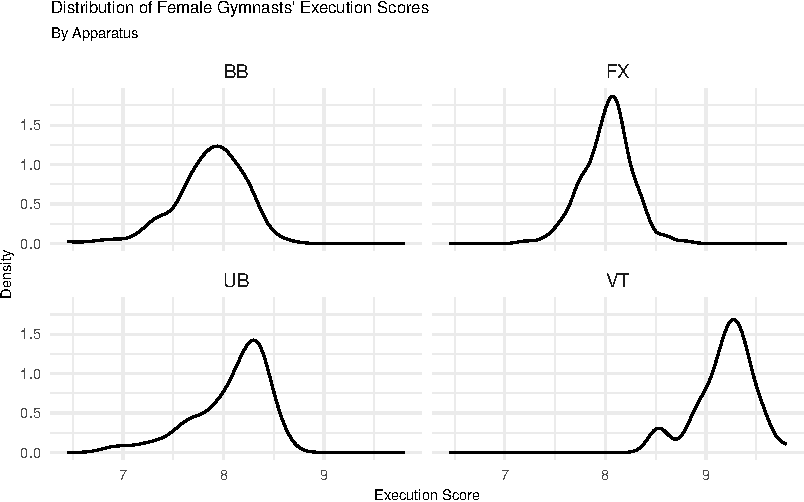
\includegraphics{Main_files/figure-pdf/execution-difficulty-distributions-1.pdf}

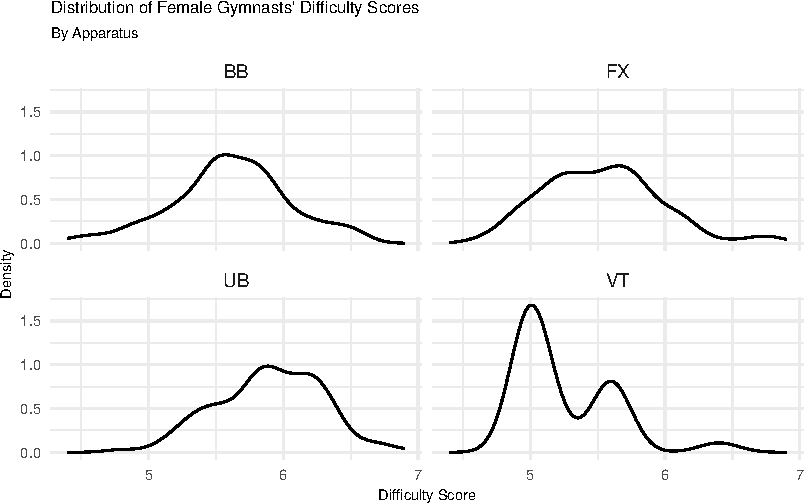
\includegraphics{Main_files/figure-pdf/execution-difficulty-distributions-2.pdf}

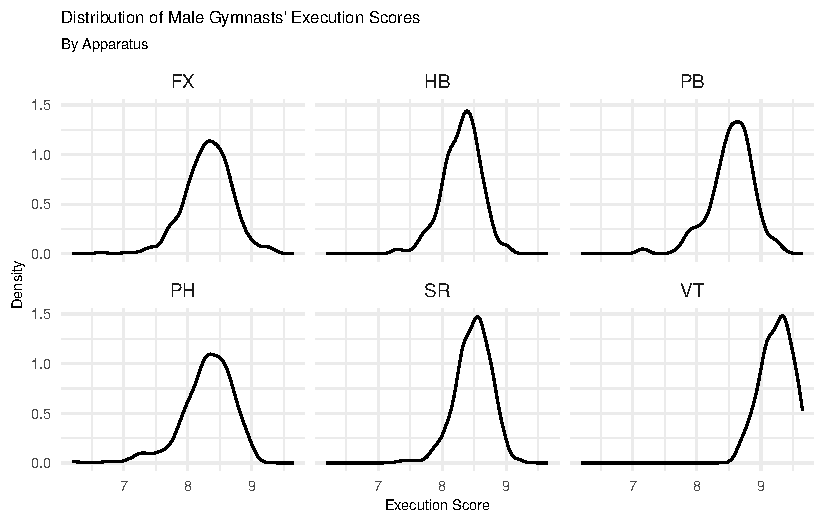
\includegraphics{Main_files/figure-pdf/execution-difficulty-distributions-3.pdf}

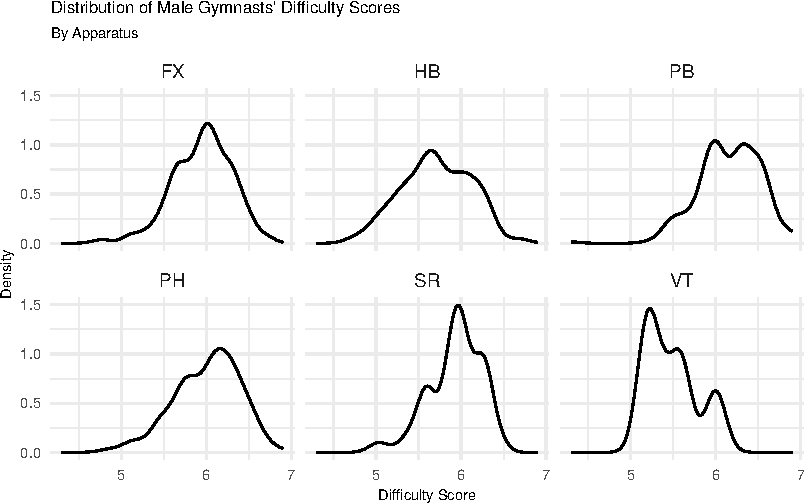
\includegraphics{Main_files/figure-pdf/execution-difficulty-distributions-4.pdf}

Additionally, we look at the distribution of mean scores and the
distribution of variance scores for men's high bar apparatus as an
example of how we will fit normal-inverse gamma priors for the means and
variances. We can see that the distribution of mean scores follows an
approximately normal distribution and the distribution of variance
scores follow an approximately inverse-gamma distribution.

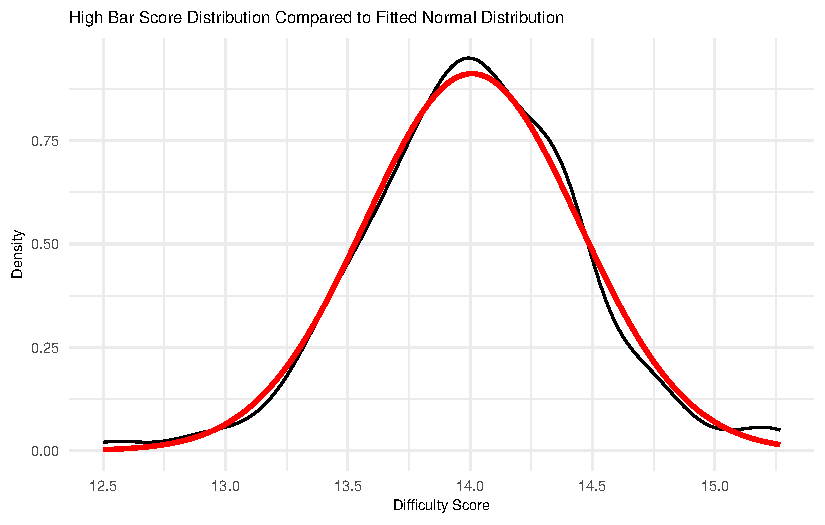
\includegraphics{Main_files/figure-pdf/highbar-fit-1.pdf}

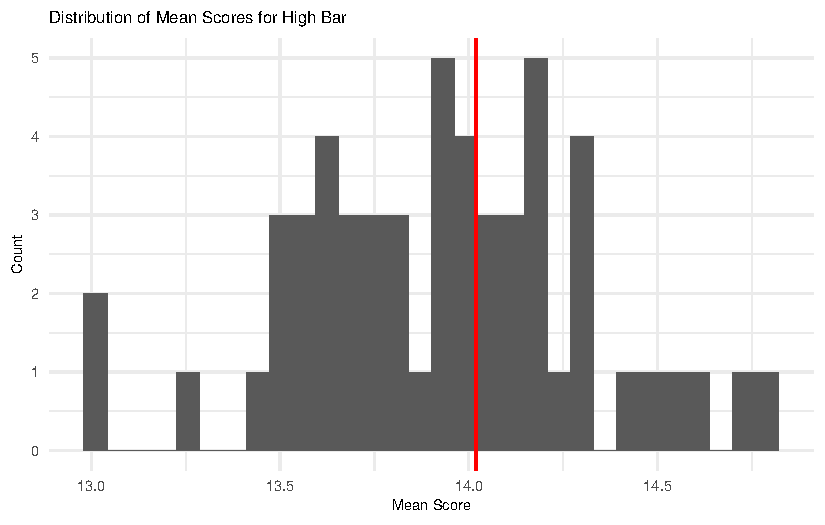
\includegraphics{Main_files/figure-pdf/scoremeans-var-1.pdf}

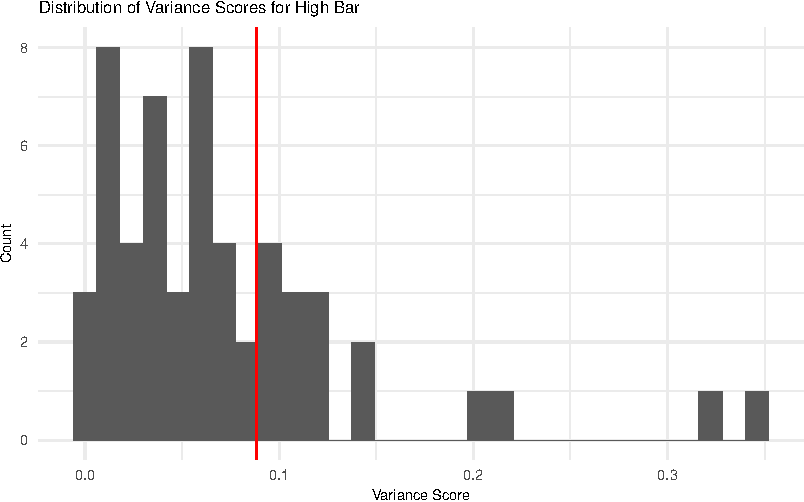
\includegraphics{Main_files/figure-pdf/scoremeans-var-2.pdf}

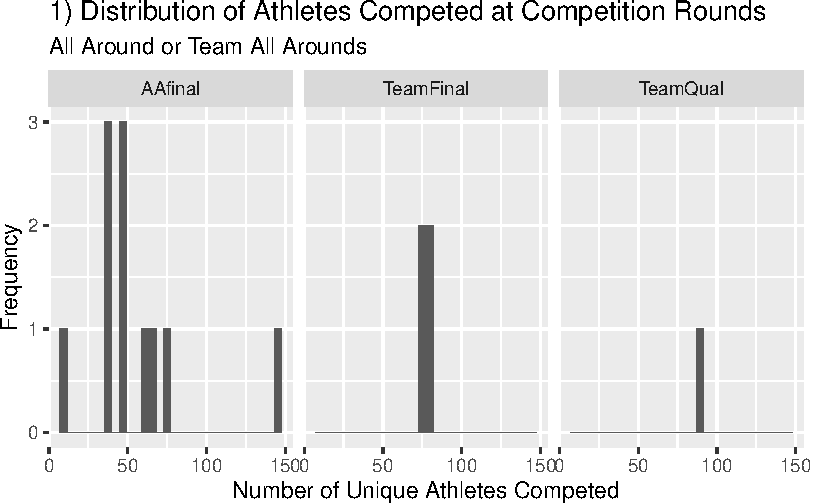
\includegraphics{Main_files/figure-pdf/unique-athletes-1.pdf}

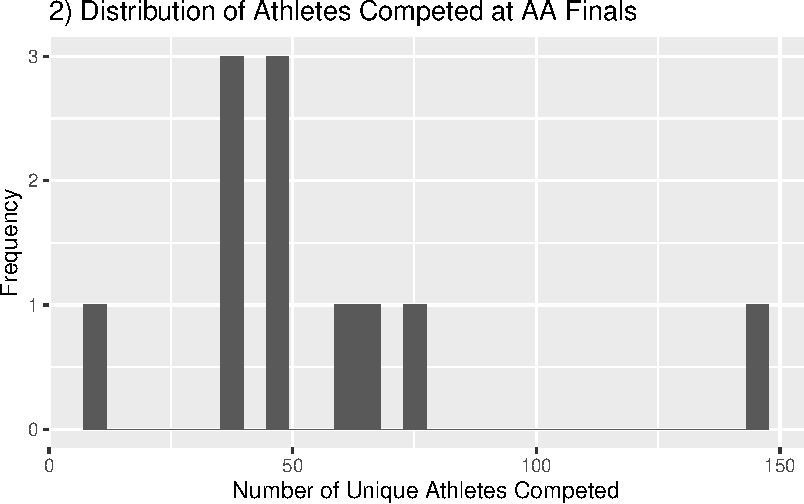
\includegraphics{Main_files/figure-pdf/unique-athletes-2.pdf}

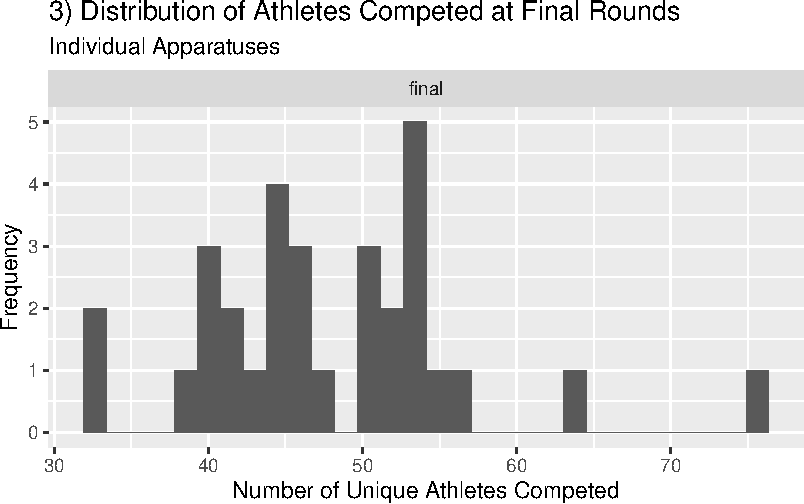
\includegraphics{Main_files/figure-pdf/unique-athletes-3.pdf}

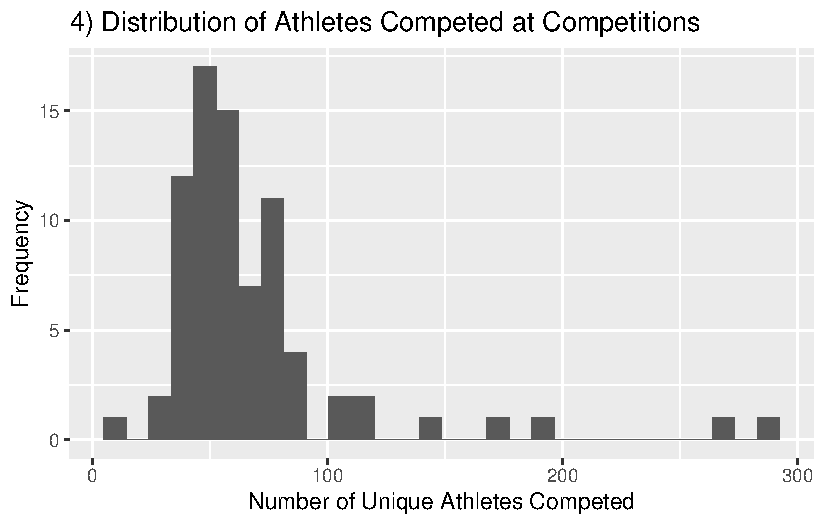
\includegraphics{Main_files/figure-pdf/unique-athletes-4.pdf}

\textbf{Image 5)}

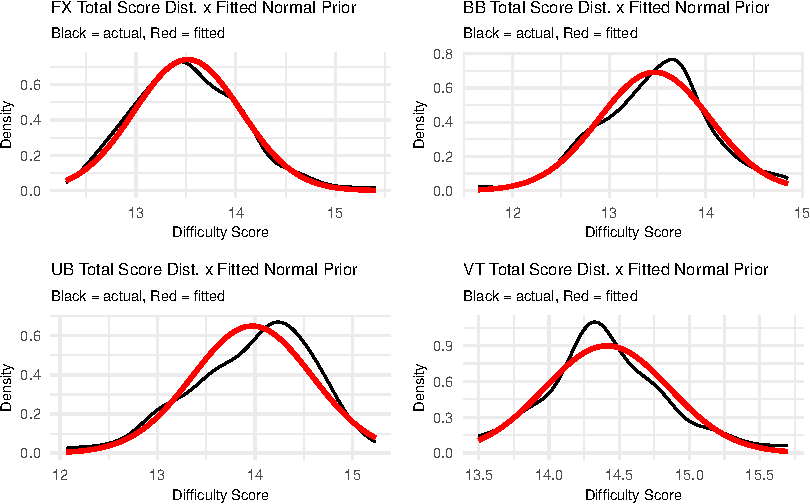
\includegraphics{Main_files/figure-pdf/unnamed-chunk-4-1.pdf}

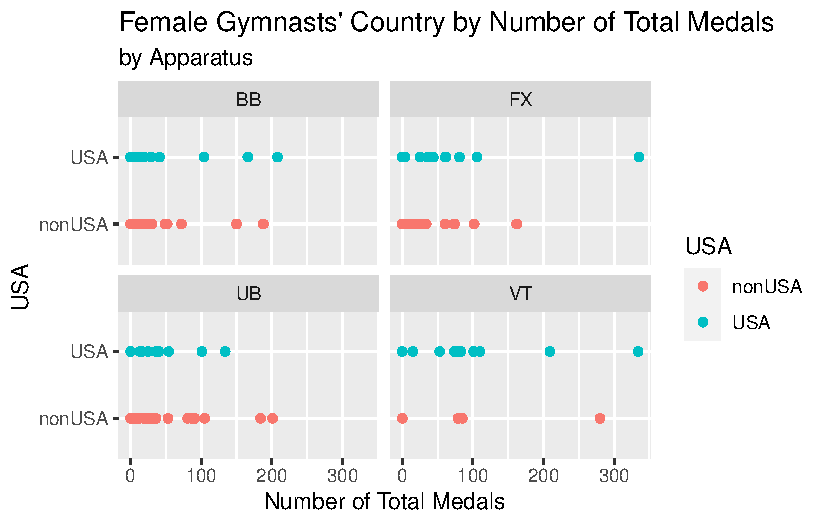
\includegraphics{Main_files/figure-pdf/unnamed-chunk-4-2.pdf}

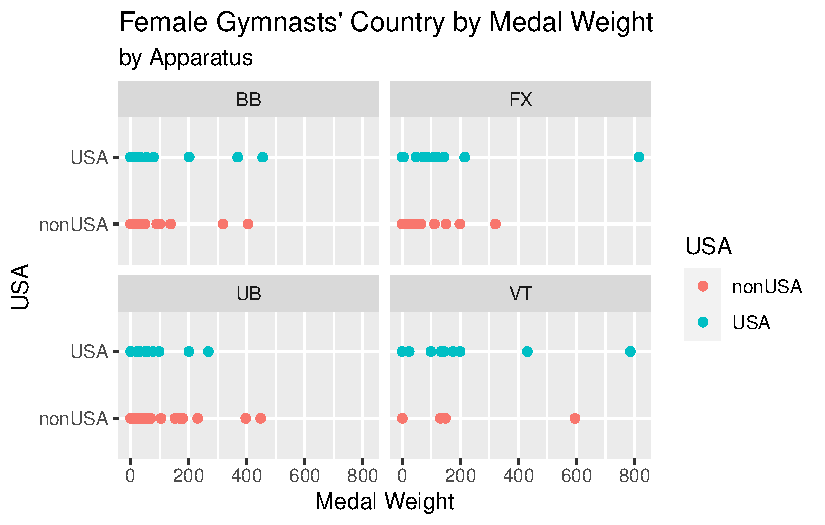
\includegraphics{Main_files/figure-pdf/unnamed-chunk-4-3.pdf}

\textbf{Image 6)}

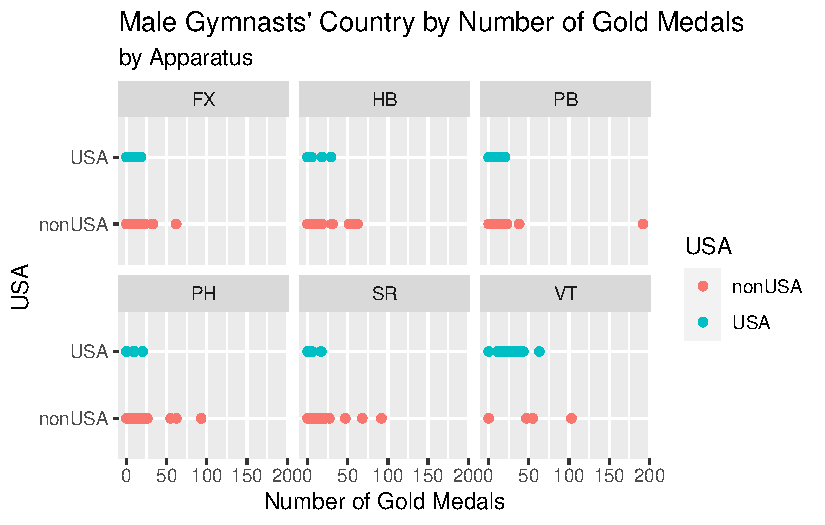
\includegraphics{Main_files/figure-pdf/unnamed-chunk-5-1.pdf}

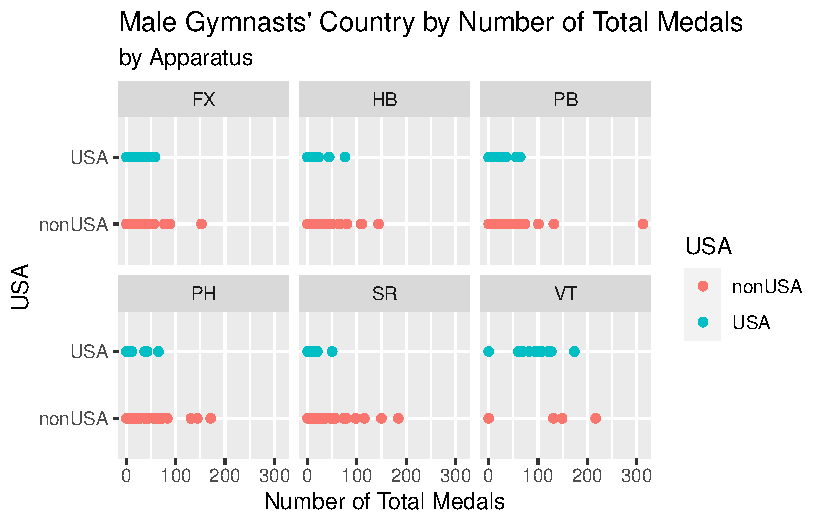
\includegraphics{Main_files/figure-pdf/unnamed-chunk-5-2.pdf}

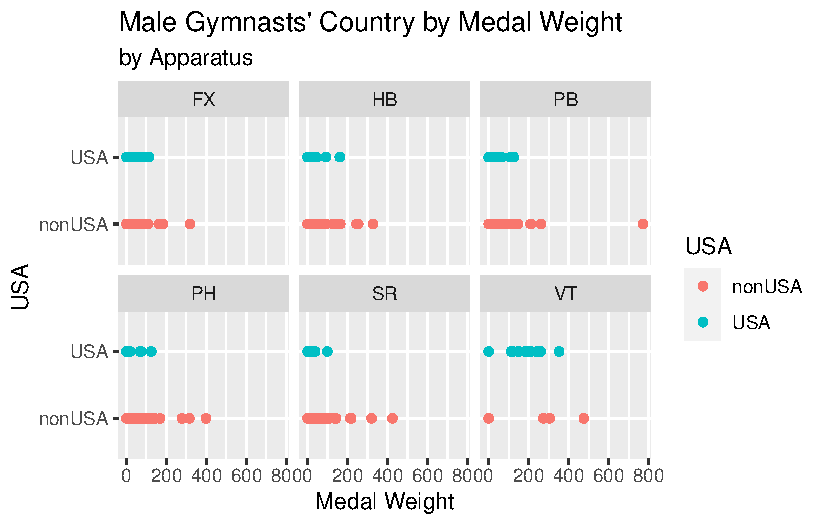
\includegraphics{Main_files/figure-pdf/unnamed-chunk-5-3.pdf}

\textbf{Image 7)}

Women:

\begin{itemize}
\item
  Top 5 athletes by apparatus for each of the 3 success metrics
\item
  Sum of each of the 3 metrics made by athletes from the US and non-US
  countries
\end{itemize}

\begin{tabular}{l|r|r|r|r|l|r|l|l}
\hline
unique\_id & Golds & Silvers & Bronzes & Total\_Medals & Country & Medal\_Weight & Apparatus & USA\\
\hline
SimBIL\_USA & 93 & 61 & 54 & 208 & USA & 455 & BB & USA\\
\hline
KonMCC\_USA & 80 & 43 & 43 & 166 & USA & 369 & BB & USA\\
\hline
YaqZHO\_CHN & 73 & 71 & 44 & 188 & CHN & 405 & BB & nonUSA\\
\hline
QinZHA\_CHN & 55 & 58 & 37 & 150 & CHN & 318 & BB & nonUSA\\
\hline
SunLEE\_USA & 34 & 30 & 40 & 104 & USA & 202 & BB & USA\\
\hline
SimBIL\_USA & 206 & 68 & 61 & 335 & USA & 815 & FX & USA\\
\hline
RebAND\_BRA & 48 & 63 & 51 & 162 & BRA & 321 & FX & nonUSA\\
\hline
KalLIN\_USA & 37 & 35 & 34 & 106 & USA & 215 & FX & USA\\
\hline
JesGAD\_GBR & 30 & 36 & 36 & 102 & GBR & 198 & FX & nonUSA\\
\hline
FlaSAR\_BRA & 22 & 33 & 19 & 74 & BRA & 151 & FX & nonUSA\\
\hline
KayNEM\_ALG & 92 & 63 & 46 & 201 & ALG & 448 & UB & nonUSA\\
\hline
QiyQIU\_CHN & 72 & 69 & 43 & 184 & CHN & 397 & UB & nonUSA\\
\hline
XiaWEI\_CHN & 47 & 32 & 26 & 105 & CHN & 231 & UB & nonUSA\\
\hline
ShiJON\_USA & 44 & 46 & 44 & 134 & USA & 268 & UB & USA\\
\hline
ZoeMIL\_USA & 37 & 26 & 38 & 101 & USA & 201 & UB & USA\\
\hline
SimBIL\_USA & 176 & 100 & 58 & 334 & USA & 786 & VT & USA\\
\hline
RebAND\_BRA & 108 & 99 & 73 & 280 & BRA & 595 & VT & nonUSA\\
\hline
JadCAR\_USA & 74 & 74 & 61 & 209 & USA & 431 & VT & USA\\
\hline
ShiJON\_USA & 29 & 31 & 50 & 110 & USA & 199 & VT & USA\\
\hline
SkyBLA\_USA & 22 & 16 & 36 & 74 & USA & 134 & VT & USA\\
\hline
\end{tabular}

\begin{tabular}{l|r|r|r|r|l|r|l|l}
\hline
unique\_id & Golds & Silvers & Bronzes & Total\_Medals & Country & Medal\_Weight & Apparatus & USA\\
\hline
SimBIL\_USA & 93 & 61 & 54 & 208 & USA & 455 & BB & USA\\
\hline
YaqZHO\_CHN & 73 & 71 & 44 & 188 & CHN & 405 & BB & nonUSA\\
\hline
KonMCC\_USA & 80 & 43 & 43 & 166 & USA & 369 & BB & USA\\
\hline
QinZHA\_CHN & 55 & 58 & 37 & 150 & CHN & 318 & BB & nonUSA\\
\hline
SunLEE\_USA & 34 & 30 & 40 & 104 & USA & 202 & BB & USA\\
\hline
SimBIL\_USA & 206 & 68 & 61 & 335 & USA & 815 & FX & USA\\
\hline
RebAND\_BRA & 48 & 63 & 51 & 162 & BRA & 321 & FX & nonUSA\\
\hline
KalLIN\_USA & 37 & 35 & 34 & 106 & USA & 215 & FX & USA\\
\hline
JesGAD\_GBR & 30 & 36 & 36 & 102 & GBR & 198 & FX & nonUSA\\
\hline
JadCAR\_USA & 18 & 27 & 36 & 81 & USA & 144 & FX & USA\\
\hline
KayNEM\_ALG & 92 & 63 & 46 & 201 & ALG & 448 & UB & nonUSA\\
\hline
QiyQIU\_CHN & 72 & 69 & 43 & 184 & CHN & 397 & UB & nonUSA\\
\hline
ShiJON\_USA & 44 & 46 & 44 & 134 & USA & 268 & UB & USA\\
\hline
XiaWEI\_CHN & 47 & 32 & 26 & 105 & CHN & 231 & UB & nonUSA\\
\hline
ZoeMIL\_USA & 37 & 26 & 38 & 101 & USA & 201 & UB & USA\\
\hline
SimBIL\_USA & 176 & 100 & 58 & 334 & USA & 786 & VT & USA\\
\hline
RebAND\_BRA & 108 & 99 & 73 & 280 & BRA & 595 & VT & nonUSA\\
\hline
JadCAR\_USA & 74 & 74 & 61 & 209 & USA & 431 & VT & USA\\
\hline
ShiJON\_USA & 29 & 31 & 50 & 110 & USA & 199 & VT & USA\\
\hline
KonMCC\_USA & 18 & 37 & 46 & 101 & USA & 174 & VT & USA\\
\hline
\end{tabular}

\begin{tabular}{l|r|r|r|r|l|r|l|l}
\hline
unique\_id & Golds & Silvers & Bronzes & Total\_Medals & Country & Medal\_Weight & Apparatus & USA\\
\hline
SimBIL\_USA & 93 & 61 & 54 & 208 & USA & 455 & BB & USA\\
\hline
YaqZHO\_CHN & 73 & 71 & 44 & 188 & CHN & 405 & BB & nonUSA\\
\hline
KonMCC\_USA & 80 & 43 & 43 & 166 & USA & 369 & BB & USA\\
\hline
QinZHA\_CHN & 55 & 58 & 37 & 150 & CHN & 318 & BB & nonUSA\\
\hline
SunLEE\_USA & 34 & 30 & 40 & 104 & USA & 202 & BB & USA\\
\hline
SimBIL\_USA & 206 & 68 & 61 & 335 & USA & 815 & FX & USA\\
\hline
RebAND\_BRA & 48 & 63 & 51 & 162 & BRA & 321 & FX & nonUSA\\
\hline
KalLIN\_USA & 37 & 35 & 34 & 106 & USA & 215 & FX & USA\\
\hline
JesGAD\_GBR & 30 & 36 & 36 & 102 & GBR & 198 & FX & nonUSA\\
\hline
FlaSAR\_BRA & 22 & 33 & 19 & 74 & BRA & 151 & FX & nonUSA\\
\hline
KayNEM\_ALG & 92 & 63 & 46 & 201 & ALG & 448 & UB & nonUSA\\
\hline
QiyQIU\_CHN & 72 & 69 & 43 & 184 & CHN & 397 & UB & nonUSA\\
\hline
ShiJON\_USA & 44 & 46 & 44 & 134 & USA & 268 & UB & USA\\
\hline
XiaWEI\_CHN & 47 & 32 & 26 & 105 & CHN & 231 & UB & nonUSA\\
\hline
ZoeMIL\_USA & 37 & 26 & 38 & 101 & USA & 201 & UB & USA\\
\hline
SimBIL\_USA & 176 & 100 & 58 & 334 & USA & 786 & VT & USA\\
\hline
RebAND\_BRA & 108 & 99 & 73 & 280 & BRA & 595 & VT & nonUSA\\
\hline
JadCAR\_USA & 74 & 74 & 61 & 209 & USA & 431 & VT & USA\\
\hline
ShiJON\_USA & 29 & 31 & 50 & 110 & USA & 199 & VT & USA\\
\hline
KonMCC\_USA & 18 & 37 & 46 & 101 & USA & 174 & VT & USA\\
\hline
\end{tabular}

\begin{tabular}{l|r|r|r}
\hline
USA & sumGolds & sumTotal & sumWeighted\\
\hline
nonUSA & 938 & 3140 & 6135\\
\hline
USA & 1062 & 2860 & 5865\\
\hline
\end{tabular}

For the women's simulation when looking at the top 5 athletes by:

\begin{itemize}
\item
  \emph{Gold Medal Count} for each apparatus there are 10 out of 20 from
  the US: balance beam (BB): 3, floor exercise (FX): 3, uneven bars
  (UB): 2, and vault (VT): 2

  \begin{itemize}
  \tightlist
  \item
    USA makes up 51\% of the total women's gold medals in the
    simulation.
  \end{itemize}
\item
  \emph{Total Medal Count} for each apparatus there are 12 out of 20
  from the US: balance beam (BB): 3, floor exercise (FX): 4, uneven bars
  (UB): 1, vault (VT): 4

  \begin{itemize}
  \tightlist
  \item
    USA makes up 47\% of the total women's medals in the simulation.
  \end{itemize}
\item
  \emph{Weighted Medal Count} for each apparatus there are 10 out of 20
  from the US: balance beam (BB): 3, floor exercise (FX): 2, uneven bars
  (UB): 1, vault (VT): 4

  \begin{itemize}
  \tightlist
  \item
    USA makes up 48\% of the weight of women's medals in the simulation.
  \end{itemize}
\end{itemize}

\textbf{Image 8)}

Men:

\begin{itemize}
\item
  Top 5 athletes by apparatus for each of the 3 success metrics
\item
  Sum of each of the 3 metrics made by athletes from the US and non-US
  countries
\end{itemize}

\begin{tabular}{l|r|r|r|r|l|r|l|l}
\hline
unique\_id & Golds & Silvers & Bronzes & Total\_Medals & Country & Medal\_Weight & Apparatus & USA\\
\hline
CarYUL\_PHI & 62 & 43 & 47 & 152 & PHI & 319 & FX & nonUSA\\
\hline
ArtDOL\_ISR & 33 & 29 & 26 & 88 & ISR & 183 & FX & nonUSA\\
\hline
RyoDOI\_JPN & 32 & 21 & 24 & 77 & JPN & 162 & FX & nonUSA\\
\hline
BohZHA\_CHN & 23 & 10 & 13 & 46 & CHN & 102 & FX & nonUSA\\
\hline
DaiHAS\_JPN & 19 & 15 & 22 & 56 & JPN & 109 & FX & nonUSA\\
\hline
KazMIN\_JPN & 19 & 16 & 8 & 43 & JPN & 97 & FX & nonUSA\\
\hline
DaiHAS\_JPN & 62 & 60 & 22 & 144 & JPN & 328 & HB & nonUSA\\
\hline
ConSHI\_CHN & 57 & 30 & 23 & 110 & CHN & 254 & HB & nonUSA\\
\hline
BohZHA\_CHN & 52 & 32 & 25 & 109 & CHN & 245 & HB & nonUSA\\
\hline
WeiSU\_\_CHN & 31 & 18 & 15 & 64 & CHN & 144 & HB & nonUSA\\
\hline
WeiSUN\_CHN & 30 & 24 & 26 & 80 & CHN & 164 & HB & nonUSA\\
\hline
JinZOU\_CHN & 192 & 75 & 46 & 313 & CHN & 772 & PB & nonUSA\\
\hline
LukDAU\_GER & 38 & 53 & 41 & 132 & GER & 261 & PB & nonUSA\\
\hline
BohZHA\_CHN & 38 & 33 & 30 & 101 & CHN & 210 & PB & nonUSA\\
\hline
CarYUL\_PHI & 23 & 27 & 23 & 73 & PHI & 146 & PB & nonUSA\\
\hline
BlaSUN\_USA & 20 & 21 & 23 & 64 & USA & 125 & PB & USA\\
\hline
MaxWHI\_GBR & 93 & 41 & 37 & 171 & GBR & 398 & PH & nonUSA\\
\hline
NarKUR\_KAZ & 62 & 47 & 35 & 144 & KAZ & 315 & PH & nonUSA\\
\hline
ChiLEE\_TPE & 55 & 37 & 39 & 131 & TPE & 278 & PH & nonUSA\\
\hline
RhyMCC\_IRL & 26 & 33 & 24 & 83 & IRL & 168 & PH & nonUSA\\
\hline
AhmABU\_JOR & 25 & 20 & 28 & 73 & JOR & 143 & PH & nonUSA\\
\hline
YanLIU\_CHN & 92 & 57 & 35 & 184 & CHN & 425 & SR & nonUSA\\
\hline
XinLAN\_CHN & 68 & 34 & 48 & 150 & CHN & 320 & SR & nonUSA\\
\hline
JinZOU\_CHN & 47 & 22 & 29 & 98 & CHN & 214 & SR & nonUSA\\
\hline
ElePET\_GRE & 27 & 49 & 39 & 115 & GRE & 218 & SR & nonUSA\\
\hline
SalMAR\_ITA & 22 & 18 & 33 & 73 & ITA & 135 & SR & nonUSA\\
\hline
JakJAR\_GBR & 103 & 53 & 61 & 217 & GBR & 476 & VT & nonUSA\\
\hline
AshHON\_USA & 63 & 52 & 59 & 174 & USA & 352 & VT & USA\\
\hline
DaiHAS\_JPN & 55 & 46 & 48 & 149 & JPN & 305 & VT & nonUSA\\
\hline
BohZHA\_CHN & 47 & 48 & 36 & 131 & CHN & 273 & VT & nonUSA\\
\hline
DonWHI\_USA & 43 & 47 & 37 & 127 & USA & 260 & VT & USA\\
\hline
\end{tabular}

\begin{tabular}{l|r|r|r|r|l|r|l|l}
\hline
unique\_id & Golds & Silvers & Bronzes & Total\_Medals & Country & Medal\_Weight & Apparatus & USA\\
\hline
CarYUL\_PHI & 62 & 43 & 47 & 152 & PHI & 319 & FX & nonUSA\\
\hline
ArtDOL\_ISR & 33 & 29 & 26 & 88 & ISR & 183 & FX & nonUSA\\
\hline
RyoDOI\_JPN & 32 & 21 & 24 & 77 & JPN & 162 & FX & nonUSA\\
\hline
PauJUD\_USA & 17 & 20 & 21 & 58 & USA & 112 & FX & USA\\
\hline
DaiHAS\_JPN & 19 & 15 & 22 & 56 & JPN & 109 & FX & nonUSA\\
\hline
DaiHAS\_JPN & 62 & 60 & 22 & 144 & JPN & 328 & HB & nonUSA\\
\hline
ConSHI\_CHN & 57 & 30 & 23 & 110 & CHN & 254 & HB & nonUSA\\
\hline
BohZHA\_CHN & 52 & 32 & 25 & 109 & CHN & 245 & HB & nonUSA\\
\hline
WeiSUN\_CHN & 30 & 24 & 26 & 80 & CHN & 164 & HB & nonUSA\\
\hline
BroMAL\_USA & 29 & 27 & 20 & 76 & USA & 161 & HB & USA\\
\hline
JinZOU\_CHN & 192 & 75 & 46 & 313 & CHN & 772 & PB & nonUSA\\
\hline
LukDAU\_GER & 38 & 53 & 41 & 132 & GER & 261 & PB & nonUSA\\
\hline
BohZHA\_CHN & 38 & 33 & 30 & 101 & CHN & 210 & PB & nonUSA\\
\hline
CarYUL\_PHI & 23 & 27 & 23 & 73 & PHI & 146 & PB & nonUSA\\
\hline
BlaSUN\_USA & 20 & 21 & 23 & 64 & USA & 125 & PB & USA\\
\hline
CurPHI\_USA & 17 & 23 & 24 & 64 & USA & 121 & PB & USA\\
\hline
MaxWHI\_GBR & 93 & 41 & 37 & 171 & GBR & 398 & PH & nonUSA\\
\hline
NarKUR\_KAZ & 62 & 47 & 35 & 144 & KAZ & 315 & PH & nonUSA\\
\hline
ChiLEE\_TPE & 55 & 37 & 39 & 131 & TPE & 278 & PH & nonUSA\\
\hline
RhyMCC\_IRL & 26 & 33 & 24 & 83 & IRL & 168 & PH & nonUSA\\
\hline
AhmABU\_JOR & 25 & 20 & 28 & 73 & JOR & 143 & PH & nonUSA\\
\hline
YanLIU\_CHN & 92 & 57 & 35 & 184 & CHN & 425 & SR & nonUSA\\
\hline
XinLAN\_CHN & 68 & 34 & 48 & 150 & CHN & 320 & SR & nonUSA\\
\hline
ElePET\_GRE & 27 & 49 & 39 & 115 & GRE & 218 & SR & nonUSA\\
\hline
JinZOU\_CHN & 47 & 22 & 29 & 98 & CHN & 214 & SR & nonUSA\\
\hline
AdeASI\_TUR & 17 & 29 & 33 & 79 & TUR & 142 & SR & nonUSA\\
\hline
JakJAR\_GBR & 103 & 53 & 61 & 217 & GBR & 476 & VT & nonUSA\\
\hline
AshHON\_USA & 63 & 52 & 59 & 174 & USA & 352 & VT & USA\\
\hline
DaiHAS\_JPN & 55 & 46 & 48 & 149 & JPN & 305 & VT & nonUSA\\
\hline
BohZHA\_CHN & 47 & 48 & 36 & 131 & CHN & 273 & VT & nonUSA\\
\hline
DonWHI\_USA & 43 & 47 & 37 & 127 & USA & 260 & VT & USA\\
\hline
\end{tabular}

\begin{tabular}{l|r|r|r|r|l|r|l|l}
\hline
unique\_id & Golds & Silvers & Bronzes & Total\_Medals & Country & Medal\_Weight & Apparatus & USA\\
\hline
CarYUL\_PHI & 62 & 43 & 47 & 152 & PHI & 319 & FX & nonUSA\\
\hline
ArtDOL\_ISR & 33 & 29 & 26 & 88 & ISR & 183 & FX & nonUSA\\
\hline
RyoDOI\_JPN & 32 & 21 & 24 & 77 & JPN & 162 & FX & nonUSA\\
\hline
PauJUD\_USA & 17 & 20 & 21 & 58 & USA & 112 & FX & USA\\
\hline
DaiHAS\_JPN & 19 & 15 & 22 & 56 & JPN & 109 & FX & nonUSA\\
\hline
DaiHAS\_JPN & 62 & 60 & 22 & 144 & JPN & 328 & HB & nonUSA\\
\hline
ConSHI\_CHN & 57 & 30 & 23 & 110 & CHN & 254 & HB & nonUSA\\
\hline
BohZHA\_CHN & 52 & 32 & 25 & 109 & CHN & 245 & HB & nonUSA\\
\hline
WeiSUN\_CHN & 30 & 24 & 26 & 80 & CHN & 164 & HB & nonUSA\\
\hline
BroMAL\_USA & 29 & 27 & 20 & 76 & USA & 161 & HB & USA\\
\hline
JinZOU\_CHN & 192 & 75 & 46 & 313 & CHN & 772 & PB & nonUSA\\
\hline
LukDAU\_GER & 38 & 53 & 41 & 132 & GER & 261 & PB & nonUSA\\
\hline
BohZHA\_CHN & 38 & 33 & 30 & 101 & CHN & 210 & PB & nonUSA\\
\hline
CarYUL\_PHI & 23 & 27 & 23 & 73 & PHI & 146 & PB & nonUSA\\
\hline
BlaSUN\_USA & 20 & 21 & 23 & 64 & USA & 125 & PB & USA\\
\hline
MaxWHI\_GBR & 93 & 41 & 37 & 171 & GBR & 398 & PH & nonUSA\\
\hline
NarKUR\_KAZ & 62 & 47 & 35 & 144 & KAZ & 315 & PH & nonUSA\\
\hline
ChiLEE\_TPE & 55 & 37 & 39 & 131 & TPE & 278 & PH & nonUSA\\
\hline
RhyMCC\_IRL & 26 & 33 & 24 & 83 & IRL & 168 & PH & nonUSA\\
\hline
AhmABU\_JOR & 25 & 20 & 28 & 73 & JOR & 143 & PH & nonUSA\\
\hline
YanLIU\_CHN & 92 & 57 & 35 & 184 & CHN & 425 & SR & nonUSA\\
\hline
XinLAN\_CHN & 68 & 34 & 48 & 150 & CHN & 320 & SR & nonUSA\\
\hline
ElePET\_GRE & 27 & 49 & 39 & 115 & GRE & 218 & SR & nonUSA\\
\hline
JinZOU\_CHN & 47 & 22 & 29 & 98 & CHN & 214 & SR & nonUSA\\
\hline
AdeASI\_TUR & 17 & 29 & 33 & 79 & TUR & 142 & SR & nonUSA\\
\hline
JakJAR\_GBR & 103 & 53 & 61 & 217 & GBR & 476 & VT & nonUSA\\
\hline
AshHON\_USA & 63 & 52 & 59 & 174 & USA & 352 & VT & USA\\
\hline
DaiHAS\_JPN & 55 & 46 & 48 & 149 & JPN & 305 & VT & nonUSA\\
\hline
BohZHA\_CHN & 47 & 48 & 36 & 131 & CHN & 273 & VT & nonUSA\\
\hline
DonWHI\_USA & 43 & 47 & 37 & 127 & USA & 260 & VT & USA\\
\hline
\end{tabular}

\begin{tabular}{l|r|r|r}
\hline
USA & sumGolds & sumTot & sumWeighted\\
\hline
nonUSA & 2333 & 6716 & 13589\\
\hline
USA & 667 & 2284 & 4411\\
\hline
\end{tabular}

For the men's simulation when looking at the top 5 athletes by:

\begin{itemize}
\item
  \emph{Gold Medal Count} for each apparatus there are 5 out of 30 from
  the US: floor exercise (FX): 1, high bar (HB): 1, parallel bars (PB):
  1 pommel horse (PH): 0, still rings (SR): 0, vault (VT): 2

  \begin{itemize}
  \tightlist
  \item
    USA makes up 21\% of the total men's gold medals in the simulation.
  \end{itemize}
\item
  \emph{Total Medal Count} for each apparatus there are 4 out of 30 from
  the US: floor exercise (FX): 1, high bar (HB): 1, parallel bars (PB):
  0, pommel horse (PH): 0, still rings (SR): 0, vault (VT): 2

  \begin{itemize}
  \tightlist
  \item
    USA makes up 24\% of the total men's medals in the simulation.
  \end{itemize}
\item
  \emph{Weighted Medal Count} for each apparatus there are 4 out of 30
  from the US: floor exercise (FX): 1, high bar (HB): 1, parallel bars
  (PB): 0, pommel horse (PH): 0, still rings (SR): 0, vault (VT): 2

  \begin{itemize}
  \tightlist
  \item
    USA makes up 23\% of the weight of men's medals in the simulation.
  \end{itemize}
\end{itemize}

\textbf{Image 9)}

\begin{verbatim}
# A tibble: 41 x 5
# Groups:   Apparatus [4]
   unique_id  Golds Country Apparatus USA   
   <chr>      <dbl> <fct>   <chr>     <fct> 
 1 SimBIL_USA    93 USA     BB        USA   
 2 KonMCC_USA    80 USA     BB        USA   
 3 YaqZHO_CHN    73 CHN     BB        nonUSA
 4 QinZHA_CHN    55 CHN     BB        nonUSA
 5 SunLEE_USA    34 USA     BB        USA   
 6 YusOU__CHN    21 CHN     BB        nonUSA
 7 HuaLUO_CHN    18 CHN     BB        nonUSA
 8 UraASH_JPN    13 JPN     BB        nonUSA
 9 SkyBLA_USA    11 USA     BB        USA   
10 QiyQIU_CHN     9 CHN     BB        nonUSA
# i 31 more rows
\end{verbatim}

\textbf{Image 10)}

\begin{verbatim}
Warning: Removed 1 rows containing missing values (`geom_point()`).
\end{verbatim}

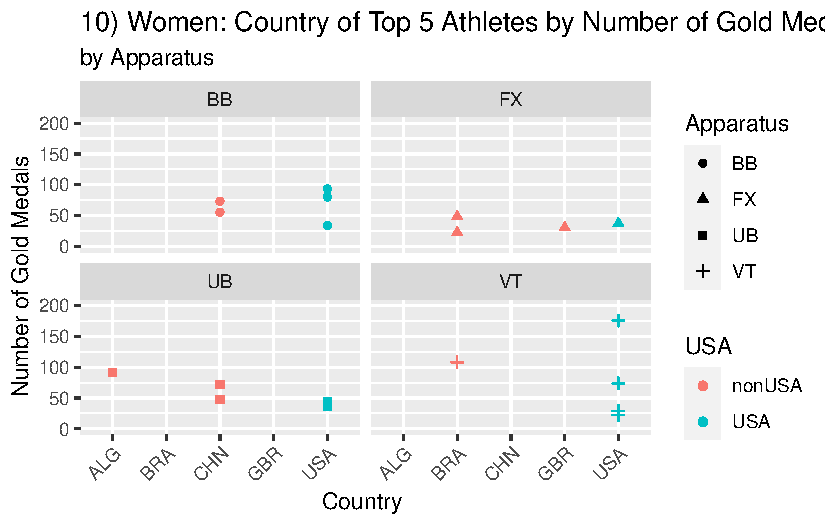
\includegraphics{Main_files/figure-pdf/unnamed-chunk-9-1.pdf}

\textbf{Image 11)}

\begin{verbatim}
# A tibble: 61 x 5
# Groups:   Apparatus [6]
   unique_id  Golds Country Apparatus USA   
   <chr>      <dbl> <fct>   <chr>     <fct> 
 1 CarYUL_PHI    62 PHI     FX        nonUSA
 2 ArtDOL_ISR    33 ISR     FX        nonUSA
 3 RyoDOI_JPN    32 JPN     FX        nonUSA
 4 BohZHA_CHN    23 CHN     FX        nonUSA
 5 DaiHAS_JPN    19 JPN     FX        nonUSA
 6 KazMIN_JPN    19 JPN     FX        nonUSA
 7 BroMAL_USA    18 USA     FX        USA   
 8 PauJUD_USA    17 USA     FX        USA   
 9 YulMOL_USA    16 USA     FX        USA   
10 GiaREG_GBR    16 GBR     FX        nonUSA
# i 51 more rows
\end{verbatim}

\textbf{Image 12)}

\begin{verbatim}
Warning: Removed 2 rows containing missing values (`geom_point()`).
\end{verbatim}

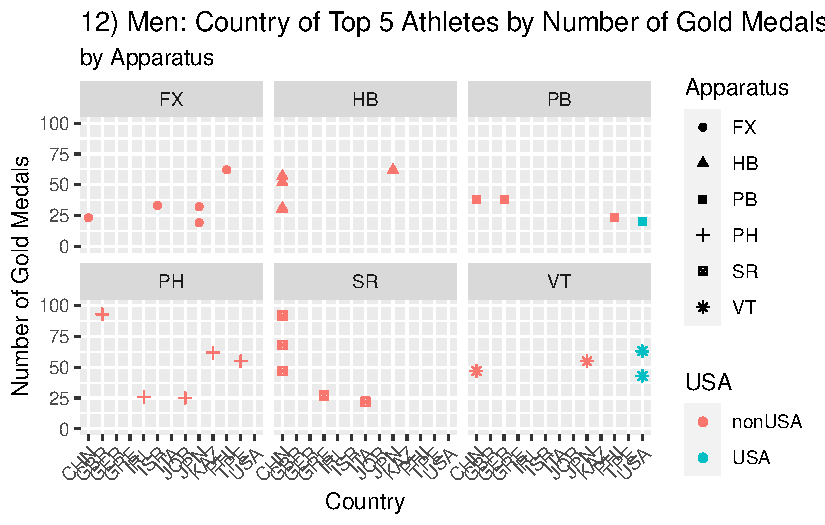
\includegraphics{Main_files/figure-pdf/unnamed-chunk-11-1.pdf}

\textbf{\emph{Note:}} The excessive number of countries display that
there is not much overlap in the top 5 most gold medal decorated
athletes on the men's team and therefore the lack of well-rounded
gymnasts.

\hypertarget{diagnostics}{%
\subsubsection{Diagnostics}\label{diagnostics}}

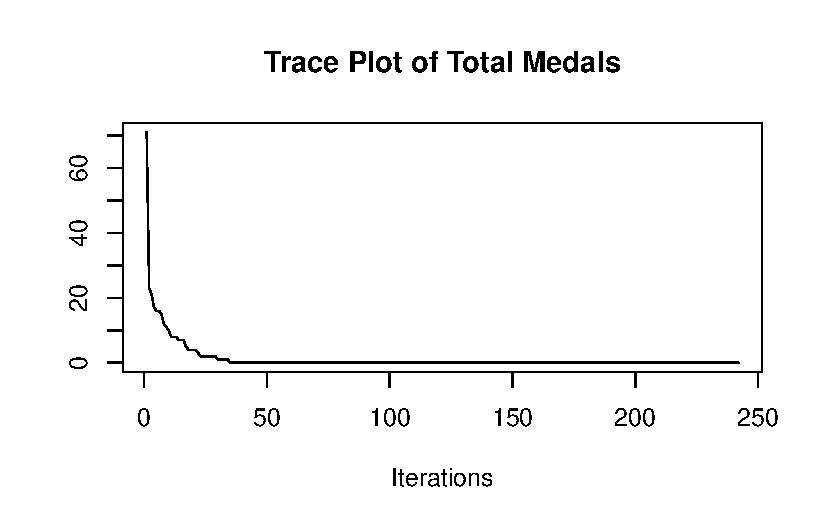
\includegraphics{Main_files/figure-pdf/unnamed-chunk-12-1.pdf}

\begin{verbatim}
    var1 
27.00493 
\end{verbatim}

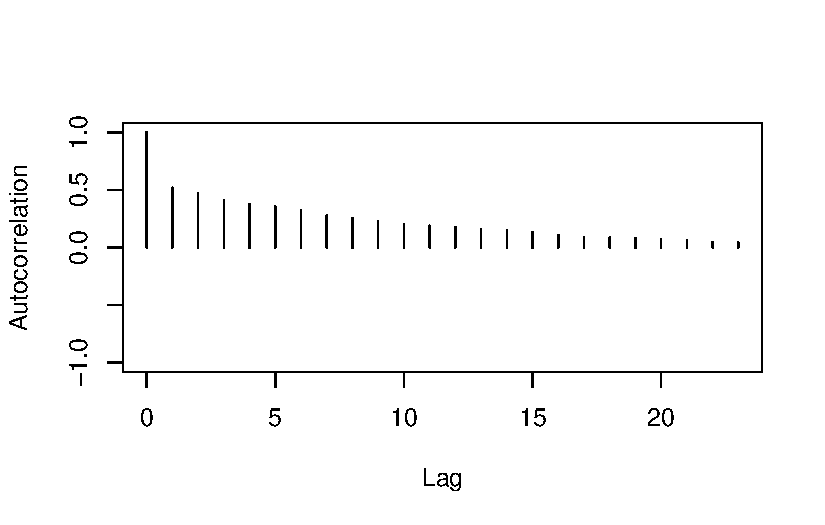
\includegraphics{Main_files/figure-pdf/unnamed-chunk-12-2.pdf}

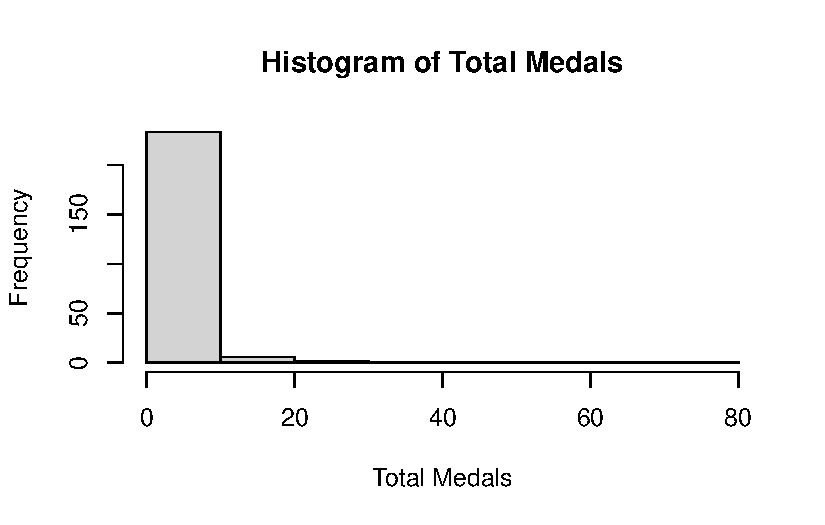
\includegraphics{Main_files/figure-pdf/unnamed-chunk-12-3.pdf}

\begin{verbatim}

Iterations = 1:968
Thinning interval = 1 
Number of chains = 1 
Sample size per chain = 968 

1. Empirical mean and standard deviation for each variable,
   plus standard error of the mean:

          Mean             SD       Naive SE Time-series SE 
        6.1983        28.0299         0.9009         2.4301 

2. Quantiles for each variable:

 2.5%   25%   50%   75% 97.5% 
 0.00  0.00  0.00  0.00 80.65 
\end{verbatim}

\begin{verbatim}
     var1 
0.1085832 
\end{verbatim}

\begin{verbatim}
    var1 
133.0432 
\end{verbatim}

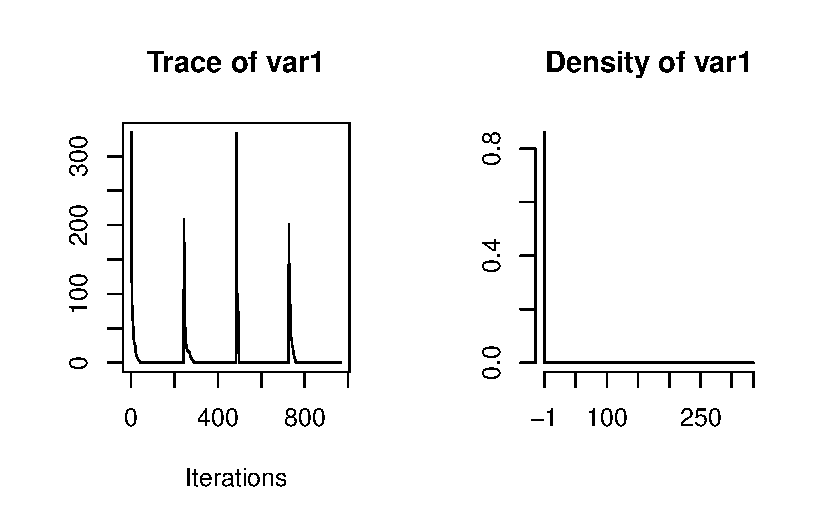
\includegraphics{Main_files/figure-pdf/unnamed-chunk-13-1.pdf}

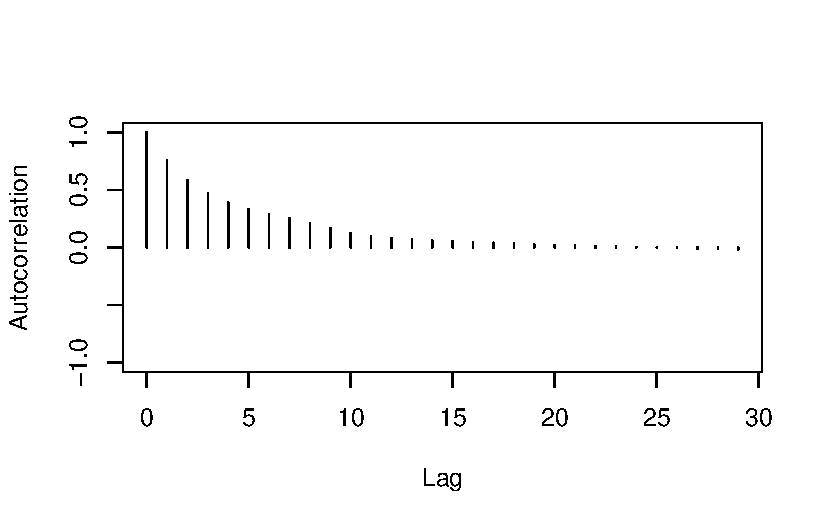
\includegraphics{Main_files/figure-pdf/unnamed-chunk-13-2.pdf}

\begin{verbatim}

Iterations = 1:1452
Thinning interval = 1 
Number of chains = 1 
Sample size per chain = 1452 

1. Empirical mean and standard deviation for each variable,
   plus standard error of the mean:

          Mean             SD       Naive SE Time-series SE 
        6.1983        22.0044         0.5775         2.1447 

2. Quantiles for each variable:

 2.5%   25%   50%   75% 97.5% 
 0.00  0.00  0.00  0.00 64.72 
\end{verbatim}

\begin{verbatim}
     var1 
0.1295658 
\end{verbatim}

\begin{verbatim}
    var1 
105.2676 
\end{verbatim}

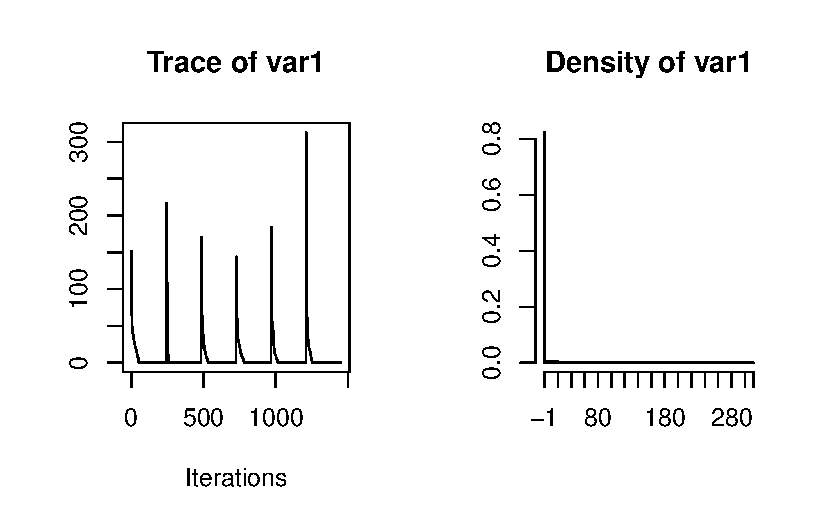
\includegraphics{Main_files/figure-pdf/unnamed-chunk-13-3.pdf}

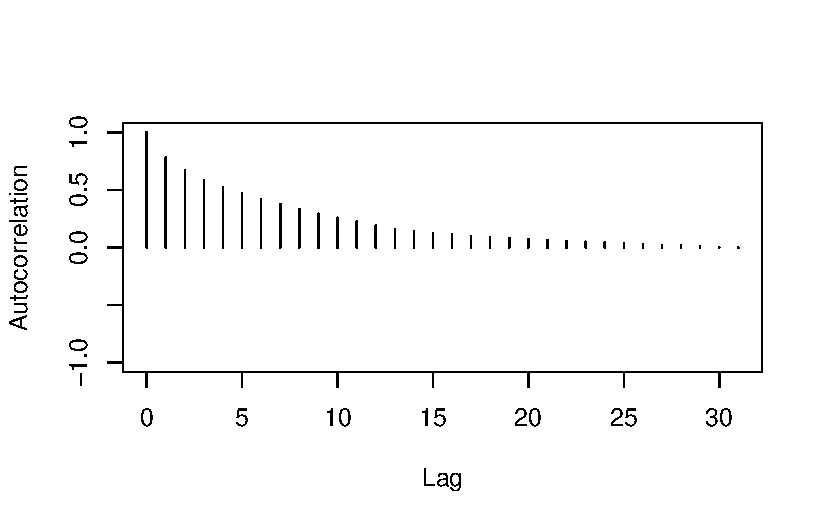
\includegraphics{Main_files/figure-pdf/unnamed-chunk-13-4.pdf}



\end{document}
